%--------------------------------------------------------------
% thesis.tex 
%--------------------------------------------------------------
% Corso di Laurea in Informatica 
% http://if.dsi.unifi.it/
% @Facolt\`a di Scienze Matematiche, Fisiche e Naturali
% @Universit\`a degli Studi di Firenze
%--------------------------------------------------------------
% - template for the main file of Informatica@Unifi Thesis 
% - based on Classic Thesis Style Copyright (C) 2008 
%   Andr\'e Miede http://www.miede.de   
%--------------------------------------------------------------
\documentclass[twoside,openright,titlepage,fleqn,
	headinclude,12pt,a4paper,BCOR5mm,footinclude]{scrbook}
%--------------------------------------------------------------
\newcommand{\myItalianTitle}{Titolo italiano\xspace}
\newcommand{\myEnglishTitle}{Titolo inglese\xspace}
% use the right myDegree option
\newcommand{\myDegree}{Corso di Laurea in Informatica\xspace}
%\newcommand{\myDegree}{
	%Corso di Laurea Specialistica in Scienze e Tecnologie 
	%dell'Informazione\xspace}
\newcommand{\myName}{Nome candidato\xspace}
\newcommand{\myProf}{Relatore\xspace}
\newcommand{\myOtherProf}{Correlatore\xspace}
\newcommand{\mySupervisor}{Nome Cognome\xspace}
\newcommand{\myFaculty}{
	Scuola di Scienze Matematiche, Fisiche e Naturali\xspace}
\newcommand{\myUni}{\protect{
	Universit\`a degli Studi di Firenze}\xspace}
\newcommand{\myLocation}{Firenze\xspace}
\newcommand{\myTime}{Anno Accademico 2018-2019\xspace}
\newcommand{\myVersion}{Version 0.1\xspace}
%--------------------------------------------------------------
\usepackage[italian]{babel}
\usepackage[latin1]{inputenc} 
\usepackage[T1]{fontenc} 
\usepackage[square,numbers]{natbib} 
\usepackage[fleqn]{amsmath}  
\usepackage{ellipsis}
\usepackage{listings}
\usepackage{subfig}
\usepackage{caption}
\usepackage{appendix}
\usepackage{siunitx}
%--------------------------------------------------------------
\usepackage{dia-classicthesis-ldpkg}
%--------------------------------------------------------------
% Options for classicthesis.sty:
% tocaligned eulerchapternumbers drafting linedheaders 
% listsseparated subfig nochapters beramono eulermath parts 
% minionpro pdfspacing
\usepackage[eulerchapternumbers,linedheaders,subfig,beramono,eulermath,
parts]{classicthesis}
%--------------------------------------------------------------
\newlength{\abcd} % for ab..z string length calculation
% how all the floats will be aligned
\newcommand{\myfloatalign}{\centering} 
\setlength{\extrarowheight}{3pt} % increase table row height
\captionsetup{format=hang,font=small}
%--------------------------------------------------------------
% Layout setting
%--------------------------------------------------------------
\usepackage{geometry}
\geometry{
	a4paper,
	ignoremp,
	bindingoffset = 1cm, 
	textwidth     = 13.5cm,
	textheight    = 21.5cm,
	lmargin       = 3.5cm, % left margin
	tmargin       = 4cm    % top margin 
}

\lstset{
  	frame=tb,
	language=Matlab,
  	aboveskip=3mm,
  	belowskip=3mm,
  	showstringspaces=false,
  	columns=flexible,
  	basicstyle={\small\ttfamily},
  	numbers=none,
  	breaklines=true,
  	breakatwhitespace=true,
  	tabsize=3
}
%--------------------------------------------------------------
\begin{document}
\frenchspacing
\raggedbottom
\pagenumbering{roman}
\pagestyle{plain}
%--------------------------------------------------------------
% Frontmatter
%--------------------------------------------------------------
%--------------------------------------------------------------
% titlepage.tex (use thesis.tex as main file)
%--------------------------------------------------------------
\begin{titlepage}
	\begin{center}
   	\large
      \hfill
      \vfill
      \begingroup
         
\includegraphics[scale=0.15]{logo/LOGO}\\
%			\spacedallcaps{\myUni} \\ 
			\myFaculty \\
			\myDegree \\ 
			\vspace{0.5cm}
         \vspace{0.5cm}    
         Tesi di Laurea    
      \endgroup 
      \vfill 
      \begingroup
      	\color{Maroon}\spacedallcaps{\myItalianTitle} \\ $\ $\\
      	\spacedallcaps{\myEnglishTitle} \\ 	
	\bigskip
      \endgroup
      \spacedlowsmallcaps{\myName}
      \vfill 
      \vfill
      Relatore: \emph{Prof. Andrea Bondavalli}\\
      Correlatore: \emph{Dott. Tommaso Zoppi}\\
      \vfill
      \vfill
      \myTime
      \vfill                      
	\end{center}        
\end{titlepage}   
%--------------------------------------------------------------
% back titlepage
%--------------------------------------------------------------
   \newpage
	\thispagestyle{empty}
	\hfill
	\vfill
	\noindent\myName: 
	\textit{\myItalianTitle,} 
	\myDegree, \textcopyright\ \myTime
%--------------------------------------------------------------
% back titlepage end
%--------------------------------------------------------------
\pagestyle{scrheadings}
%--------------------------------------------------------------
% Mainmatter
%--------------------------------------------------------------
\pagenumbering{arabic}
% use \cleardoublepage here to avoid problems with pdfbookmark
%\chapter{Introduzione}
L'Information Technology (IT) svolge un ruolo fondamentale nella vita di tutti i giorni, nel modo in cui riusciamo a relazionarci, a lavorare, a vivere la nostra quotidianeit�. L'IT permea quasi tutti i nostri comportamenti quotidiani e pu� essere considerata lo strumento pi� efficace per la creazione di ricchezza economica da parte delle aziende.\\ Grazie all'IT infatti le aziende hanno potuto generare vantaggi e sfruttare nuove opportunit�. Oggi questi vantaggi e benefici, comprensivi di applicazioni, funzionalit� e infrastrutture, sono alla portata di tutti.\\ Visto l'importante ruolo assunto dall'IT, nasce l'esigenza di preservare i sistemi informatici; a questa necessit� fa capo l'\textit{hazard analysis}, o analisi dei rischi, un processo di valutazione delle criticit� inerenti un sistema informatico.\\
Il \textbf{rischio} � la potenzialit� che un'azione o un'attivit� porti a una perdita o ad un evento indesiderabile. Quello del rischio � un concetto connesso con le aspettative umane e la loro capacit� di predizione/intervento in situazioni non note o incerte. L'uomo nel corso degli anni ha imparato a confrontarsi con il rischio con un atteggiamento di sfida, ricercando sempre pi� un equilibrio tra razionalizzazione degli eventi e utilizzo dell'intuito. Nel linguaggio comune, rischio � spesso usato come sinonimo di probabilit� di una perdita o di un pericolo/minaccia. In generale, ogni indicatore di rischio � proporzionale all'effetto atteso e alla sua probabilit� di accadimento. \cite{quattordici}\\ L'esigenza di iniziare a quantificare i rischi � nata in ambito bancario, infatti fin dal tardo medioevo i banchieri sono abituati a gestire il rischio di credito, ovvero il principale rischio a cui essi sono esposti. I banchieri lombardi che a partire dal 1100 operavano in Francia, Germania ed Inghilterra utilizzavano gi� efficaci tecniche di mitigazione del rischio di credito, quali ad esempio la richiesta di cessione in pegno di oggetti di valore.\cite{otto} \\ 
Non � possibile individuare un comportamento umano o un'attivit� naturale che non venga sottoposta a rischi temporanei o costanti; solamente le scienze pure, come la matematica o la fisica,  governate dalle ferree leggi del puro determinismo, non si confrontano con tale concetto.\\


\section{Scopo della tesi}
Gli obiettivi proposti nel lavoro di tesi sono quelli di riportare l'importanza dell'\textit{Hazard analysis} in ambito ferroviario e di applicare tale procedura all'apparato Interfaccia Mobile Remota (IMR) di RFI. Tale apparato nasce con lo scopo di migliorare e velocizzare l'esecuzione delle operazioni di manutenzione lungo le linee ferroviarie. Tramite l'IMR deve diventare possibile per un operatore, tramite un tablet, effettuare una serie di operazioni, come impedire il passaggio di treni in una zona della linea ferroviaria, senza recarsi fisicamente in stazione per ottenere l'autorizzazione. Poich� il malfunzionamento di una qualunque delle fasi dell'operazione � critica per la vita dell'operatore e per il funzionamento della linea, tale procedura remota deve essere sicura, quindi eventuali malfunzionamenti devono essere visibili per l'operatore. Grazie alla procedura di hazard analysis � stato possibile evidenziare le principali criticit� del sistema in questione e quindi ricercare una soluzione oppurtuna per ognuna di esse. % use \myChapter command instead of \chapter
\tableofcontents
\listoffigures
\cleardoublepage
\thispagestyle{empty}
\begin{flushright}
\null\vspace{\stretch {1}}
\emph{"Inserire citazione" \break --- Inserire autore citazione} \vspace{\stretch{2}}\null
\end{flushright}
\cleardoublepage
\chapter{Introduzione}
L'Information Technology (IT) svolge un ruolo fondamentale nella vita di tutti i giorni, nel modo in cui riusciamo a relazionarci, a lavorare, a vivere la nostra quotidianeit�. L'IT permea quasi tutti i nostri comportamenti quotidiani e pu� essere considerata lo strumento pi� efficace per la creazione di ricchezza economica da parte delle aziende.\\ Grazie all'IT infatti le aziende hanno potuto generare vantaggi e sfruttare nuove opportunit�. Oggi questi vantaggi e benefici, comprensivi di applicazioni, funzionalit� e infrastrutture, sono alla portata di tutti.\\ Visto l'importante ruolo assunto dall'IT, nasce l'esigenza di preservare i sistemi informatici; a questa necessit� fa capo l'\textit{hazard analysis}, o analisi dei rischi, un processo di valutazione delle criticit� inerenti un sistema informatico.\\
Il \textbf{rischio} � la potenzialit� che un'azione o un'attivit� porti a una perdita o ad un evento indesiderabile. Quello del rischio � un concetto connesso con le aspettative umane e la loro capacit� di predizione/intervento in situazioni non note o incerte. L'uomo nel corso degli anni ha imparato a confrontarsi con il rischio con un atteggiamento di sfida, ricercando sempre pi� un equilibrio tra razionalizzazione degli eventi e utilizzo dell'intuito. Nel linguaggio comune, rischio � spesso usato come sinonimo di probabilit� di una perdita o di un pericolo/minaccia. In generale, ogni indicatore di rischio � proporzionale all'effetto atteso e alla sua probabilit� di accadimento. \cite{quattordici}\\ L'esigenza di iniziare a quantificare i rischi � nata in ambito bancario, infatti fin dal tardo medioevo i banchieri sono abituati a gestire il rischio di credito, ovvero il principale rischio a cui essi sono esposti. I banchieri lombardi che a partire dal 1100 operavano in Francia, Germania ed Inghilterra utilizzavano gi� efficaci tecniche di mitigazione del rischio di credito, quali ad esempio la richiesta di cessione in pegno di oggetti di valore.\cite{otto} \\ 
Non � possibile individuare un comportamento umano o un'attivit� naturale che non venga sottoposta a rischi temporanei o costanti; solamente le scienze pure, come la matematica o la fisica,  governate dalle ferree leggi del puro determinismo, non si confrontano con tale concetto.\\


\section{Scopo della tesi}
Gli obiettivi proposti nel lavoro di tesi sono quelli di riportare l'importanza dell'\textit{Hazard analysis} in ambito ferroviario e di applicare tale procedura all'apparato Interfaccia Mobile Remota (IMR) di RFI. Tale apparato nasce con lo scopo di migliorare e velocizzare l'esecuzione delle operazioni di manutenzione lungo le linee ferroviarie. Tramite l'IMR deve diventare possibile per un operatore, tramite un tablet, effettuare una serie di operazioni, come impedire il passaggio di treni in una zona della linea ferroviaria, senza recarsi fisicamente in stazione per ottenere l'autorizzazione. Poich� il malfunzionamento di una qualunque delle fasi dell'operazione � critica per la vita dell'operatore e per il funzionamento della linea, tale procedura remota deve essere sicura, quindi eventuali malfunzionamenti devono essere visibili per l'operatore. Grazie alla procedura di hazard analysis � stato possibile evidenziare le principali criticit� del sistema in questione e quindi ricercare una soluzione oppurtuna per ognuna di esse.
\chapter{L'analisi dei rischi}
La valutazione dei rischi rappresenta il momento fondamentale per la prevenzione delle criticit� nelle aziende con lo scopo di individuare e risolvere i problemi che � possibile riscontrare.
Esistono molti strumenti e tecniche disponibili per l'identificazione di potenziali pericoli e problemi di operabilit�, di seguito sono riportate i pi� utilizzati:
\begin{itemize}
	\item \textbf{Checklists}: lista di voci che occorre controllare e spuntare per verificare che una determinata serie di operazioni sia stata eseguita correttamente;
	\item \textbf{Fault Modes and Effects Analysis (FMEA)}: analisi eseguita preventivamente e quindi basata su considerazioni teoriche e non sperimentali. Come primo passo viene effettuata la scomposizione del sistema in sottosistemi, per ognuno di essi devono essere elencati tutti i possibili guasti e successivamente le cause e le conseguenze; \cite{uno}
	\item \textbf{Fault Tree Analysis}: tecnica analitica in cui innanzitutto viene individuato uno stato indesiderato in cui pu� venire a trovarsi il sistema e in seguito viene effettuata un'analisi per determinare tutti i modi credibili in cui l'evento indesiderato pu� verificarsi. \cite{due}
	\item \textbf{Studio "What-if"}: viene condotto utilizzando un approccio del tipo brainstorming; si inizia con l'analizzare pericoli gi� noti al team di lavoro per arrivare ad altri potenziali scenari incidentali;
	\item \textbf{HAZOP}: esercizio che si svolge attraverso la formulazione di alcune specifiche domande strutturate; � finalizzato all'individuazione di deviazioni dagli intenti di progetto che possono portare ad inconvenienti di sicurezza o di esercizio. \cite{tre}
\end{itemize}

Alcune tecniche, come le Checklists e lo Studio "What-If", possono essere utilizzate all'inizio del ciclo di vita del sistema o se non � richiesta un'analisi dettagliata; al contrario, se vogliamo avere informazioni pi� complete sui pericoli a cui � sottoposto il sistema � opportuno procedere con un'analisi HAZOP, tale tecnica verr� descritta e approfondita successivamente.\
\newline
Nella seguenti tesi verr� esposta l'hazard analysis dell'apparato IMR di RFI per la manutenzione delle varie linee ferroviarie.\\
L'obiettivo del lavoro � quello di individuare tutti i potenziali pericoli, sia quelli essenzialmente rilevanti per l'area immediata del sistema, sia quelli con una sfera di influenza pi� ampia.\\
Per effettuare tale lavoro � stata utilizzata la strategia \textbf{HAZOP} (	\textbf{HAZ}ard and \textbf{OP}erability analysis); tale tecnica ha avuto origine da studi di tipo assicurativo, specie su grandi impianti di processo, estendendo la sua applicazione ad ambiti e dimensioni diverse.
L'HAZOP mira all'individuazione dei pericoli esistenti nella gestione di un determinato processo lavorativo. Tali pericoli sono identificati e indagati sulla base di deviazioni, siano esse accidentali o meno, di parametri chiave, caratteristici del processo in esame. \cite{tre}\\
L'espressione \textit{analisi dei rischi} viene sinteticamente utilizzata per indicare un processo che in pratica comprende 4 fasi:
\begin{itemize}
	\item \textit{Definizione}: in questa fase gli obiettivi e lo scopo dell'analisi devono essere definiti. Questa prima fase � fondamentale per chiarire quali siano i confini del sistema e le sue interfacce con altri sistemi, in modo tale che l'analisi non si discosti in aree irrilevanti rispetto all'obiettivo;
	\item \textit{Preparazione}: questa fase ha lo scopo di ottenere le informazioni necessarie per effettuare l'analisi e di convertire tali informazioni in un formato adatto. In seguito deve essere riportata una descrizione del progetto contenente tutti i dettagli tecnici e amministrativi necessari. Devono essere fornite informazioni circa le condizioni ambientali in cui il sistema operer�, qualifiche, abilit� ed esperienza del personale operativo e di manutenzione e infine devono essere riportate le problematiche evidenziate in sistemi simili. Non di minore importanza � l'operazione di stima del tempo necessario per condurre l'analisi che deve essere eseguita in questo frangente; infine, devono essere scelte le parole guida pi� adeguate per condurre l'analisi del sistema, considerando che una parola guida troppo specifica pu� limitare le idee e la discussione, al contrario una troppo generica potrebbe non focalizzare lo studio in modo efficiente. Di seguito � riportata la lista delle parole guida:
	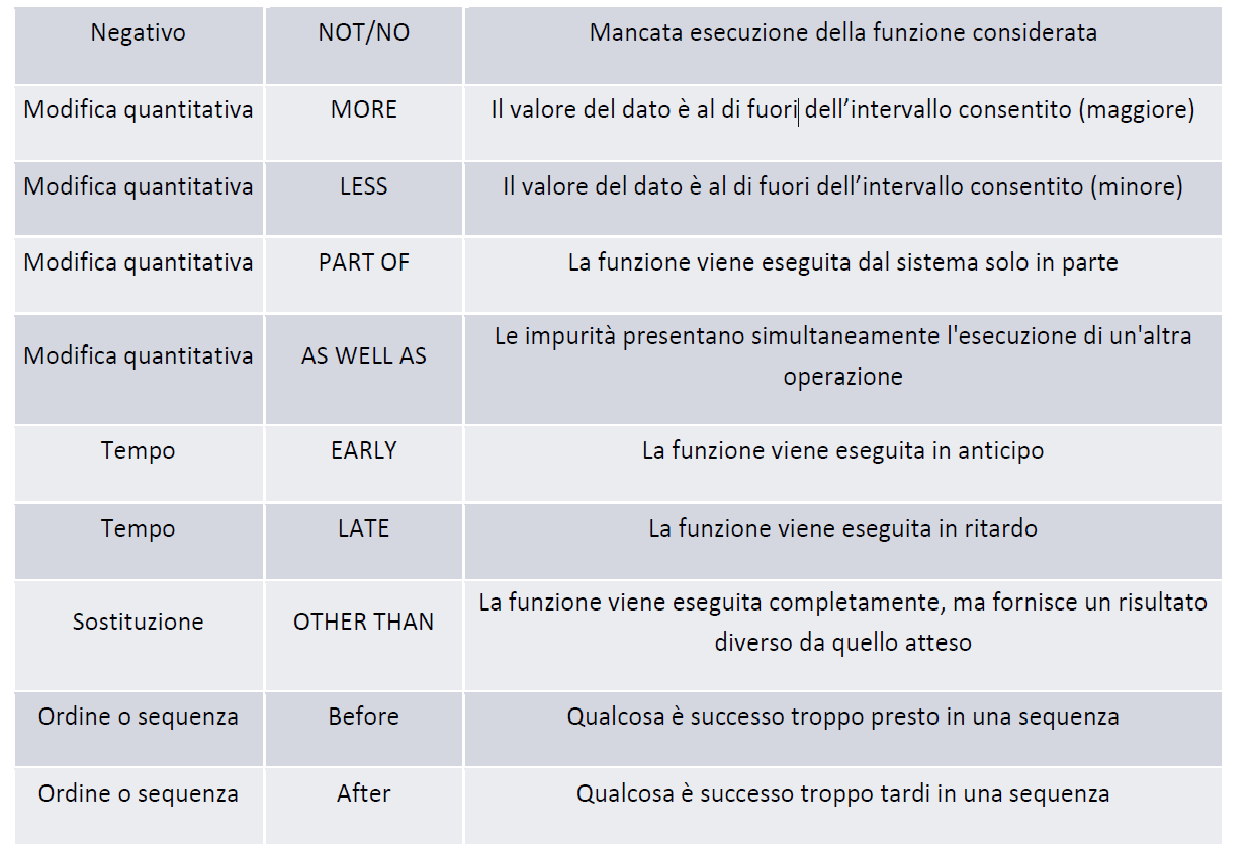
\includegraphics[scale = 0.5]{img/parolechiave}
	\item \textit{Esaminazione}: questa � la fase che rappresenta la vera e propria analisi del sistema. Come prima cosa viene diviso il sistema in parti, tale divisione deve essere effettuata in modo pertinente ai fini dell'analisi; in seguito deve essere spiegato il ruolo progettuale della parte in questione, gli elementi pertinenti e le eventuali caratteristiche associate agli elementi identificati.
	Per ogni parte del sistema devono essere individuate le parole guida appropriate, ovvero quelle che possono dar luce a eventuali criticit�. Le parole guida vengono esaminate nel contesto dell'elemento o della caratteristica studiata per rilevare eventuali deviazioni credibili dall'intento progettuale.\\ 
	Qualora venga trovata una deviazione credibile, viene effettuata un'indagine per individuare tutte le cause e le conseguenze. Le deviazioni vengono classificate in base al potenziale impatto e alla loro frequenza di accadimento, come vedremo in seguito. Di fondamentale importanza � identificare la presenza di meccanismi di protezione e rilevamento della deviazione che possono essere inclusi nella parte selezionata. Questo procedimento viene ripetuto per ogni parte del sistema, per ogni parola guida e per ogni sua interpretazione, al fine di riuscire a individuare tutti i rischi a cui il sistema pu� andare incontro.\\
	Quando una parte � stata del tutto esaminata, dovrebbe essere contrassegnata come completata. Di seguito viene riportato il diagramma di flusso della procedura appena descritta:\\
	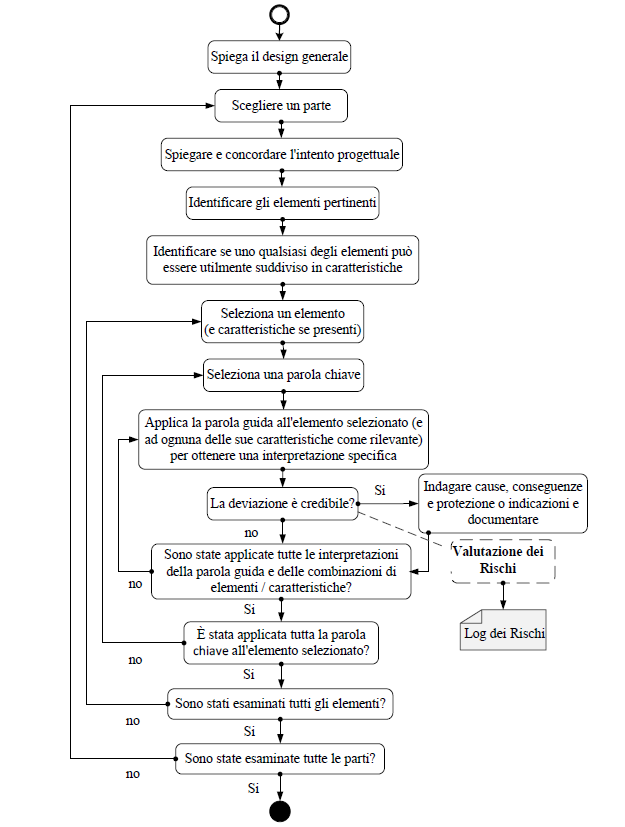
\includegraphics{img/diagrammaesame}
	\item \textit{Documentazione}: per completare l'analisi e ottenere tutti i suoi benefici � opportuno documentarla. Esistono due approcci per effettuare tale procedura: registrazione completa o solo per eccezione. La registrazione completa comporta la registrazione di tutti i risultati. Questo metodo pu� risultare ingombrante ma sicuramente completo di tutte le informazioni; al contrario, la registrazione delle eccezioni implica la memorizzazione esclusivamente dei rischi identificati e dei problemi di operabilit�. In tal caso la quantit� di dati da memorizzare � inferiore e sicuramente la gestione di questi ultimi � pi� semplice.\\ Una buona documentazione dovrebbe includere dettagliatamente quanto segue:
	\begin{itemize}
		\item dettagli dei pericoli identificati e problemi di operabilit�;
		\item raccomandazioni per eventuali ulteriori studi su aspetti specifici del progetto utilizzando tecniche diverse, se necessario;
		\item azioni necessarie per affrontare le problematiche individuate durante lo studio;
		\item un elenco di tutte le parti considerate nell'analisi, insieme alla motivazione associata all'eventuale esclusione di determinate parti del sistema;
		\item elenco di tutti i disegni, specifiche, schede tecniche, report, ecc...
	\end{itemize}
 Attraverso la registrazione per eccezioni le informazioni sui vari rischi sono descritte in maniera piuttosto concisa, senza riportare informazioni dettagliate.\\
 Nella documentazione ogni azzardo, problema operativo o pericolo, insieme alle proprie eventuali cause, dovrebbe essere registrato come elemento separato e indipendente.\\ Infine, dovrebbe essere adottato un sistema di numerazione per fare in modo che ogni rischio, problema operativo, mitigazione e raccomandazione venga identificato in maniera univoca. Per garantire il recupero della documentazione, � opportuno che essa venga archiviata.
\end{itemize}
 \subsection{Il processo per la valutazione del rischio}
 Come precedentemente anticipato nella fase di esaminazione � opportuno effettuare una valutazione del rischio riscontrato. \\
 \begin{figure}[htbp]
 	\centering
 	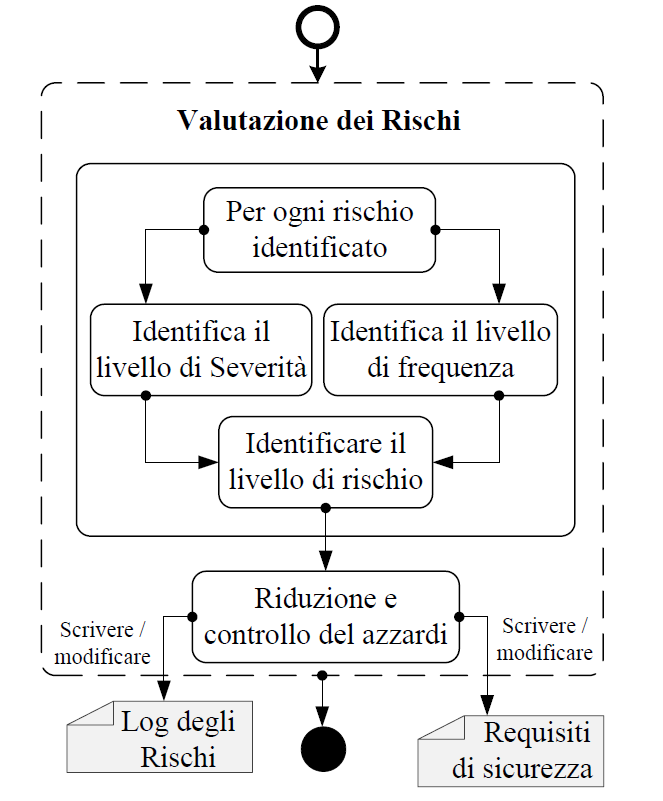
\includegraphics[scale=0.4]{img/valrischi}
 	\caption{Il processo per la valutazione dei rischi}
 \end{figure}
Le attivit� di valutazione del rischio vengono condotte con lo scopo di quantificare il rischio associato ad ogni pericolo. Per ogni comportamento anomalo individuato viene analizzata la frequenza di occorrenza e la sua severit�. Dal connubio di queste informazioni � possibile identificare il livello del rischio. 
\begin{figure}[htbp]
	\centering
	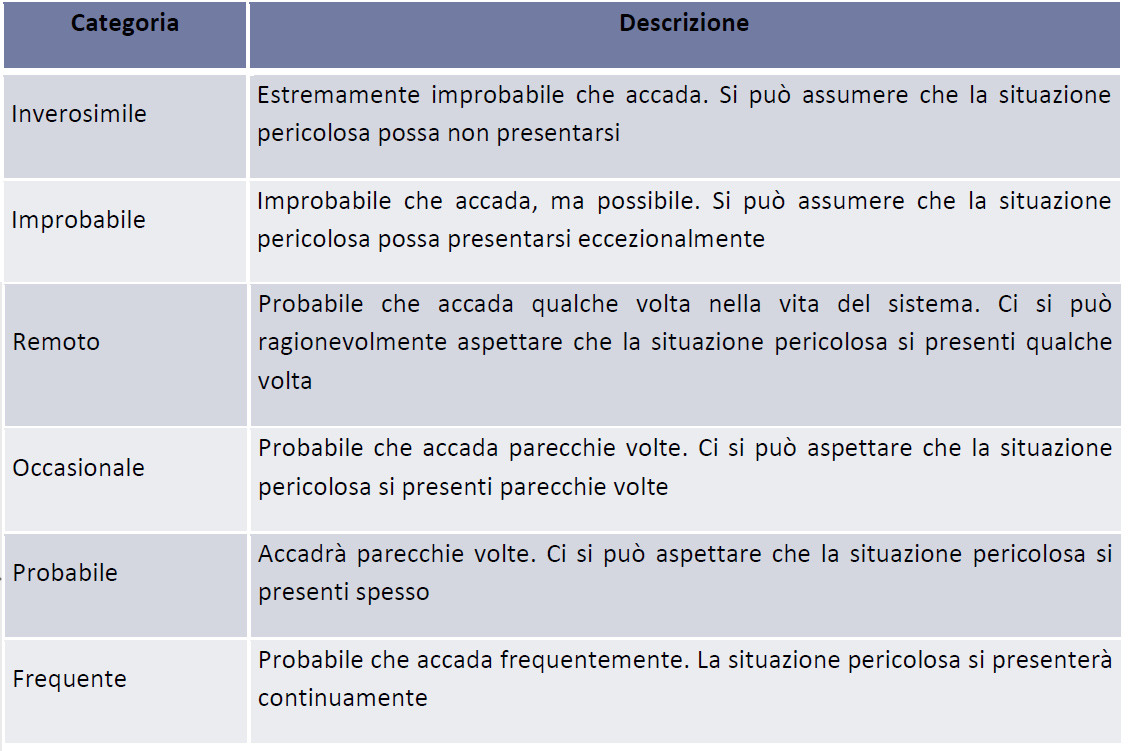
\includegraphics[scale=0.4]{img/frequenza}\\
	\caption{Tabella per la classificazione delle frequenze}
\end{figure}


\begin{figure}[htbp]
	\centering
	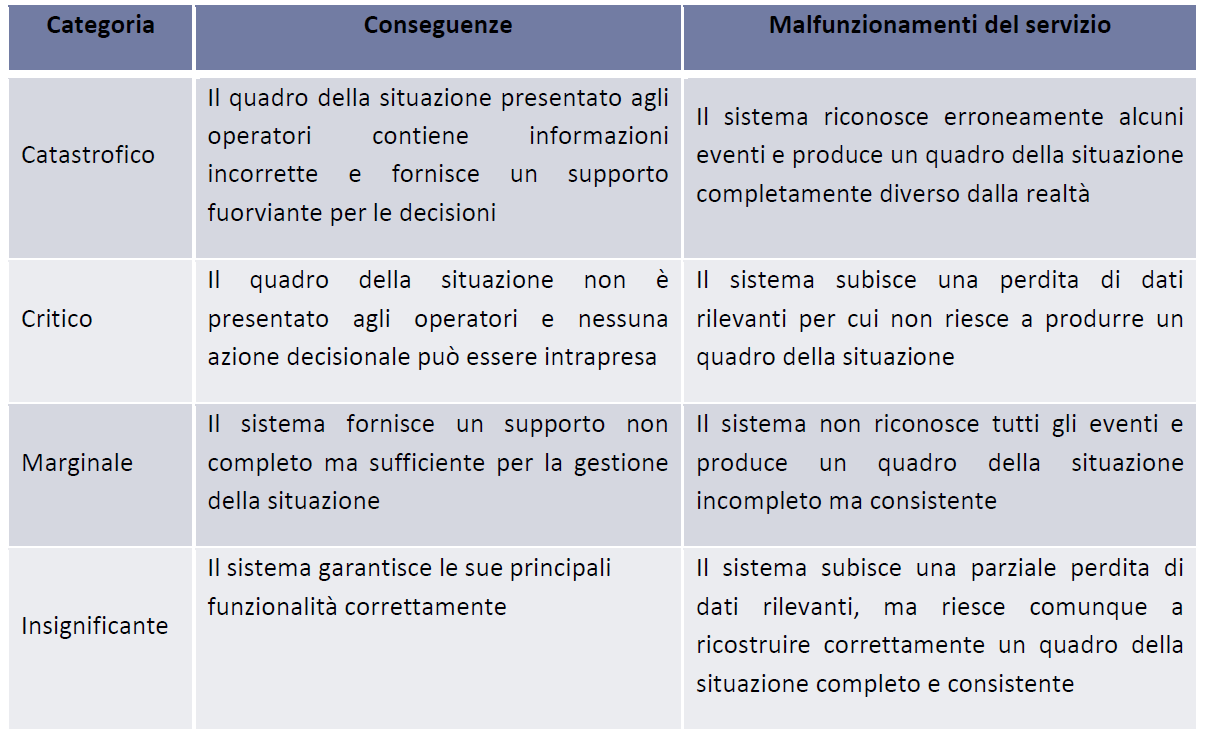
\includegraphics[scale=0.4]{img/severit}\\
	\caption{Tabella per la classificazione della severit�}
\end{figure}
Quest'ultimo pu� essere classificato come:
\begin{itemize}
	\item trascurabile
	\item tollerabile
	\item indesiderabile
	\item intollerabile.
\end{itemize} 
Qualora il livello del rischio sia trascurabile o tollerabile non � necessario individuare un'opportuna mitigazione, in quanto il verificarsi del rischio non viene ritenuto pericoloso nei confronti del sistema, ugualmente se l'incombensa del pericolo � altamente improbabile. Negli altri casi l'analisi procede con la ricerca dell'opportuna soluzione che avr� come scopo o ridurre la severit� del rischio oppure la sua frequenza di occorrenza.

	\begin{figure}[htbp]
		\centering
		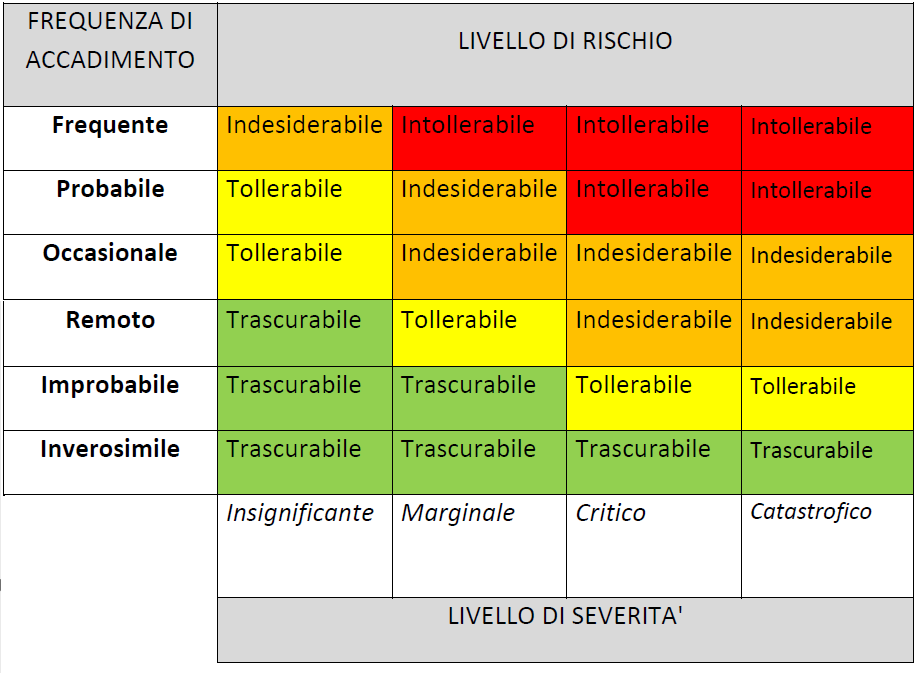
\includegraphics[scale=0.4]{img/risklevel}\\
		\caption{Risk Matrix}
	\end{figure}
	
 


\chapter{L'apparato IMR (Interfaccia Mobile Remota)}


L'apparato IMR di RFI nasce con lo scopo di migliorare e velocizzare l'esecuzione delle operazioni di manutenzione lungo le varie linee ferroviarie; tramite questo apparato molte operazioni vengono remotizzate, dando la possibilit� all'operatore, tramite il tablet, di eseguire una serie di comandi senza recarsi fisicamente in stazione.

\section{Apparati centrali}
Per assegnare a ciascun treno il percorso previsto nelle stazioni, nei bivi o nelle altre localit� di servizio, � necessario predisporre gli scambi nella posizione voluta, assicurarsi che il percorso del treno non abbia interferenze con il percorso di altri treni e che sia libero nel momento programmato. Queste condizioni si concretizzano attraverso impianti tecnologici di varie generazioni: gli Apparati Centrali. Scopo degli Apparati Centrali di una tratta, a prescindere dalla tecnologia utilizzata, � garantire la movimentazione in sicurezza dei treni, sia in stazione che durante il percorso.\\L'\textbf{apparato centrale elettrico a itinerari} (ACEI) realizza l'itinerario in sicurezza attraverso un unico comando impartito mediante un pulsante o una tastiera dal DM (Dirigente Movimento). Alcuni di questi apparati sono comandabili a distanza e quindi rendono possibile la gestione di pi� stazioni o di una intera linea contemporanteamente. \\L'\textbf{apparato centrale computerizzato} (ACC) rappresenta l'evoluzione tecnologica degli Apparati Centrali realizzati con tecnologia tradizionale elettromeccanica, come l'ACEI.
Con l'introduzione degli apparati ACC infatti le apparecchiature elettromeccaniche vengono sostituite con analoghi dispositivi elettronici, realizzati con componenti sia hardware che software, in grado comunque di garantire i medesimi livelli di sicurezza. Attraverso l'ACC vengono introdotti adeguati strumenti di diagnostica automatizzata che permettono al personale della manutenzione di effettuare le operazioni correttive necessarie in caso di guasto in tempi notevolmente ridotti rispetto alla soluzione elettromeccanica utilizzata precedentemente. \cite{cinque}
\begin{figure}
	\centering
	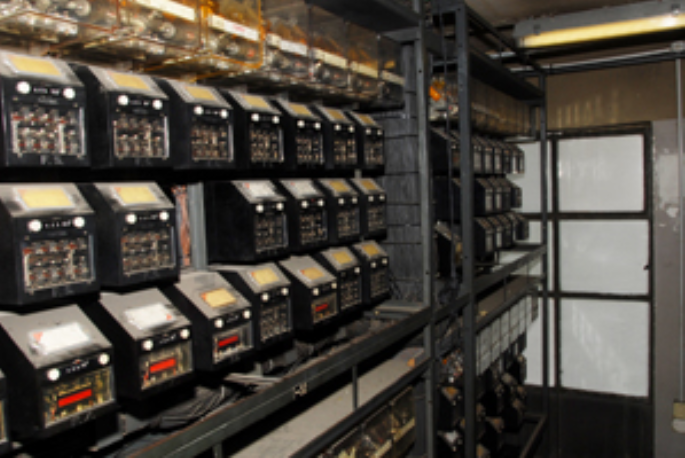
\includegraphics[scale=0.5]{img/apparaticentrali}
	\caption{Apparati centrali}
\end{figure}


\section{La manutenzione della linea ferroviaria}
Prima di introdurre la descrizione dell'apparato IMR, � opportuno delineare come opera il sistema RFI di Manutenzione della Linea.\\
Ogni stazione ferroviaria pu� essere considerata divisa in zone, ciascuna rappresentante una specifica sezione: la loro visualizzazione in una singola immagine viene detta sinottico.\\
Ogni zona pu� essere considerata indipendente dalle altre zone confinanti, infatti, qualora si renda necessario un intervento di manutenzione, � possibile impedire il passaggio dei treni esclusivamente in quella data sezione. Tale operazione viene gestita tramite l'armadio chiavi di zona, ovvero un pannello contenente tutte le chiavi delle zone. Una chiave non inserita nel pannello indica la non agibilit� della zona per qualunque operazione che non sia di manutenzione.\\
Ad esempio, supponiamo che sia necessario effettuare operazioni di manutenzione nella zona \textit{x}, l'operatore si reca all'armadio chiavi di zona, prende la chiave \textit{x}, la sfila dal pannello e la tiene con s� fino alla fine delle operazioni di manutenzione. Una volta concluse tali operazioni, l'operatore torna in stazione e ripone la chiave nell'armadio chiavi di zona.\\
Il problema ricorrente � che l'armadio spesso � lontano dal luogo in cui deve essere eseguita la manutenzione, quindi, all'operatore occorre spesso troppo  tempo per prendere la chiave e riporla.\\Di seguito � riportata la procedura completa per la rimozione di una chiave dall'armadio:
\begin{enumerate}
	\item chiedere l'autorizzazione al guardiano dell'armadio;
	\item fare una mezza rotazione della chiave sull'armadio;
	\item chiamare l'autorit� centrale per chiedere l'autorizzazione;
	\item staccare la chiave e iniziare le operazioni di manutenzione\cite{nove}.
	
\end{enumerate}


\section{L'apparato IMR}

L'apparato IMR nasce con lo scopo di evitare che l'operatore debba andare fisicamente all'armadio chiavi di zona a prelevare la chiave necessaria per effettuare le operazioni di manutenzione.\\
RFI vuole fare in modo che il sistema di terra ACEI/ACC comunichi con il nuovo dispositivo IMR. La funzione di questo apparato � quella di fornire connettivit� all'ACEI/ACC che � attualmente isolato. Il tablet  comunicher� quindi con il dispositivo IMR e quest'ultimo inoltrer� i comandi agli apparati ACEI/ACC.\\
Dato che il malfunzionamento di una qualunque operazione � critico per la vita dell'operatore e per il corretto funzionamento della linea, tale procedura remota deve essere eseguita in completa sicurezza ed eventuali malfunzionamenti devono essere visibili per l'operatore. A tale scopo � opportuno procedere con una dettagliata analisi dei rischi.\\


\section{Architettura IMR}
L' architettura Terra-Tablet dell'apparato IMR evidenzia due zone distinte:

\begin{itemize}
	\item un'area non sicura, comprendente il Tablet e i server IMRG e IMRW, potenzialmente esposti a minacce dannose e che non sono costruiti per soddisfare qualsiasi vincolo di sicurezza;
	\item un'area sicura, comprendente il server locale IMRS e gli enti di stazione. Tutte le azioni che avvengono in tale zona funzionano in conformit� con il SIL con cui sono state certificate, con una probabilit� di guasti catastrofici ragionevolmente bassa.
\end{itemize}  
\begin{figure}
	\centering
	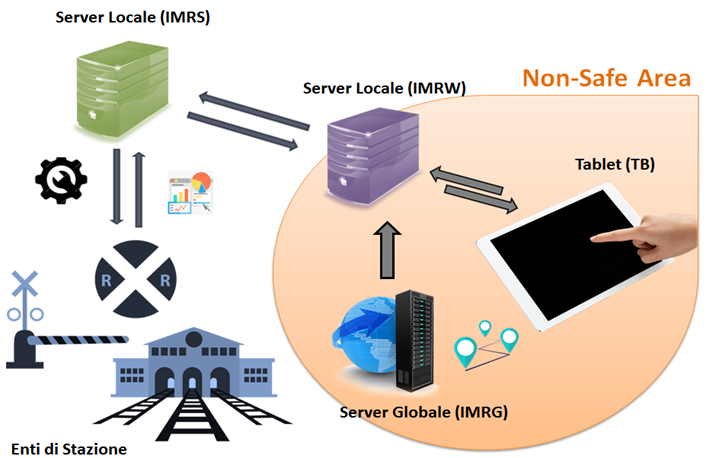
\includegraphics[scale=0.7]{img/architettura}
	\caption{Architettura IMR}
\end{figure}

\subsection{Tablet Operatore}

Ogni addetto AM viene dotato di un tablet TB commerciale per consentire la remotizzazione delle operazioni che richiederebbero l'accesso fisico all'armadio chiavi di zona.\\
Come evidenziato dall'immagine, il tablet si trova nell'area non sicura e pertanto le azioni eseguite devono essere rigorosamente regolamentate per evitare problemi di safety. Il dispositivo mobile esegue una Web App tramite la quale il manutentore potr� comunicare con l'apparato di terra e potr� inviare comandi e visualizzare lo stato della linea e degli enti.
\subsection{Server IMRG}
Tale componente si trova nell'area non sicura, � un server generico senza nessun vincolo di safety o security. Le due uniche funzioni di IMRG sono:
\begin{itemize}
	\item effettuare un reindirizzamento iniziale dell'AM all'IMRW corretto in base alla stazione che l'AM seleziona,
	\item fungere da repository condivisa delle chiavi pubbliche degli agenti di manutenzione.
\end{itemize} 
\subsection{Server IMRW}
Tale componente, come i due appena descritti, si trova nella zona non sicura dell'architettura. Il ruolo del server � quello di esporre i servizi web che possono essere chiamati remotamente dagli utenti e di assemblare le pagine web sulla base dei dati forniti da IMRS.
\subsection{Server IMRS}
Questo server sicuro gestisce, controlla, valida e verifica le interazioni tra l'operatore e gli apparati computerizzati di stazione. Tale componente � progettato, sviluppato e certificato SIL4, si trova infatti nella zona sicura.\\
Le principali funzioni sono di seguito elencate:
\begin{itemize}
	\item gestire l'autenticazione,
	\item controllare i comandi inviati dall'AM e comunicare con gli attuatori
	\item memorizzare dati critici
	\item comunicare con l'IMRW, fornendogli i dati necessari all'assemblaggio delle pagine web necessarie.
\end{itemize}


\section{Procedura di Connessione}
Di seguito � riportata la procedura di connessione del tablet:
\begin{enumerate}
	\item l'agente di manutenzione (AM), dopo aver acceso il Tablet ed aperto la Web App, specifica la stazione in cui sta operando;\\
	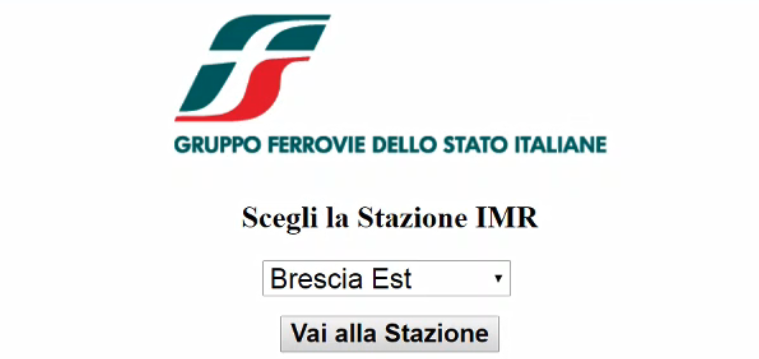
\includegraphics[scale=0.5]{img/sceglistazione}
	\item il Tablet chiede al server globale IMRG l'indirizzo del server locale IMRW relativo alla stazione in cui l'AM deve eseguire le operazioni di manutenzione;
	\item una volta che l'AM ottiene l'indirizzo del server di stazione, viene stabilita automaticamente una connessione punto-punto diretta con IMRW;
	\item l'AM immette le informazioni per l'autenticazione sul server locale: qualcosa che sa (la password) e qualcosa che possiede (la chiave privata);\\
		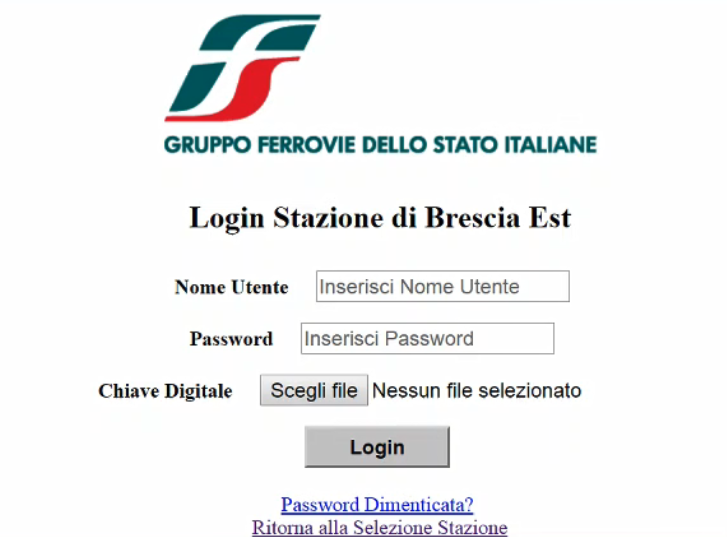
\includegraphics[scale=0.5]{img/login}
	\item la coppia unsername-password viene crittografata utilizzando la chiave privata e inviata al server locale IMRW, che la reinoltra al server sicuro IMRS, assieme all'elenco delle chiavi pubbliche memorizzate su IMRG;
	\item l'autenticazione viene interamente eseguita su IMRS;
	\item se la fase di autenticazione � andata a buon fine, verr� inviata la schermata del Terminale Operatore sul Tablet.
\end{enumerate}
\begin{figure}[ht]
	\centering
	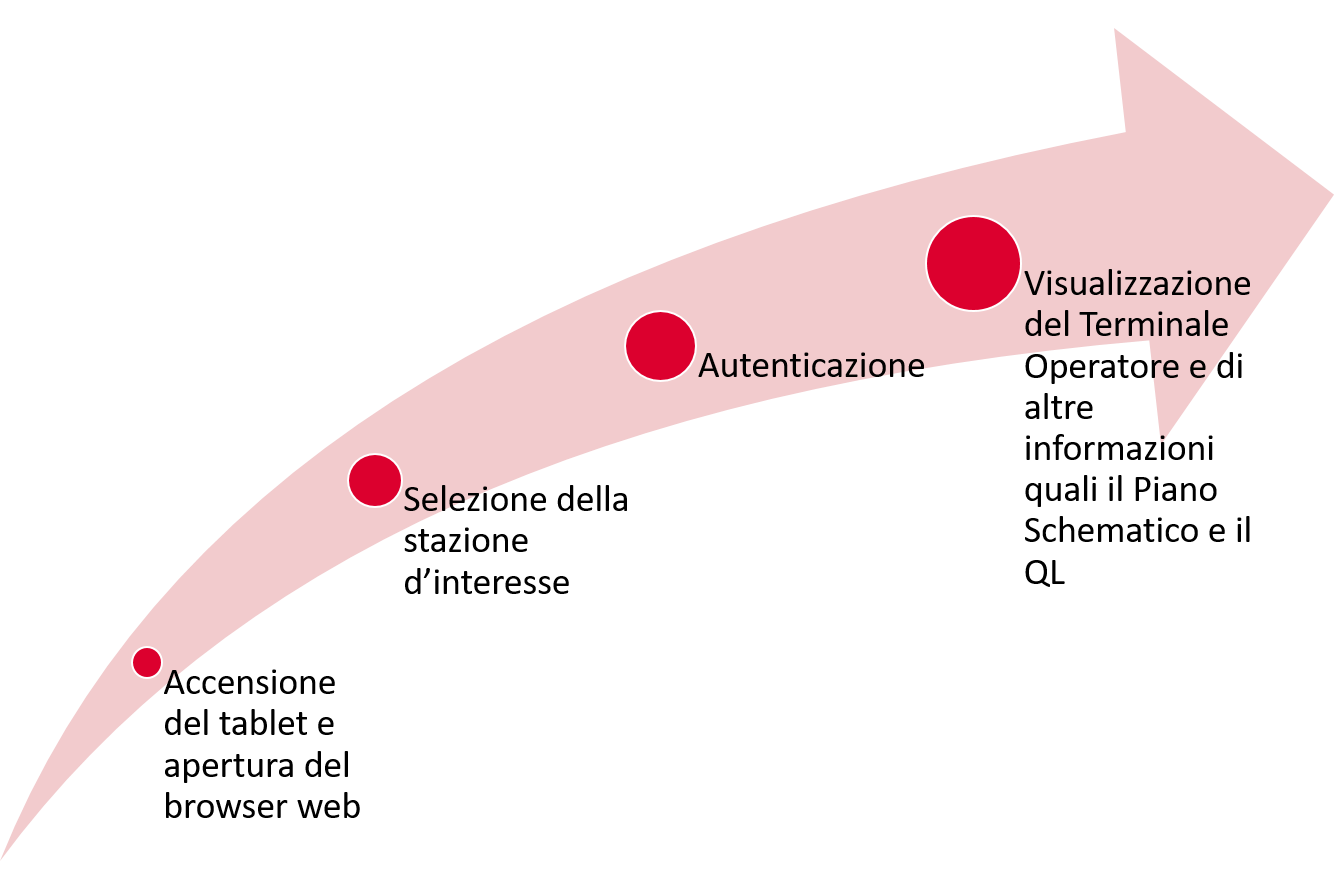
\includegraphics[scale=0.3]{img/procedura}
	\caption{Procedura di Connessione}
\end{figure}

\subsection{Funzionalit� del Terminale Operatore}
Il Terminale Operatore (TO) � lo strumento attraverso il quale un operatore � in grado di comunicare con l'apparato centrale ACC/ACEI, inoltrando comandi e ricevendo informazioni utili sullo stato del sistema. Dal TO devono essere attivabili principalmente le seguenti funzioni:
\begin{itemize}
	\item Funzioni di Movimento (formazione itinerari, formazione istradamenti, etc);
	\item Funzioni di Ente (manovra deviatoio, esclusione ente, soccorsi, etc);
	\item Funzioni di Soccorso mirate per i Movimenti;
	\item Funzioni per la gestione delle Anormalit� e degli Allarmi;
	\item Funzioni per la messaggistica e la modulistica.
\end{itemize}
A ciascuna categoria di funzioni � associato uno specifico men�, a cui corrisponde un sottomen�, pi� o meno articolato a seconda del tipo di funzione. Al fine di rendere pi� immediata possibile la scelta delle funzioni da eseguire, l'accesso ai men� � possibile attraverso icone che determinano l'apertura delle maschere corrispondenti.\\
Nello specifico, le icone presenti nella schermata Terminale Operatore rappresentano i seguenti enti:
\begin{itemize}
	\item	DV - Deviatoio
	\item	SCF - Scarpa Fermacarri
	\item	SE - Segnale Alto
	\item	TCH - Posto a Terra
	\item	CDB - Circuito di Binario di Stazione
	\item	CDBL - Corcuito di Binario di Linea
	\item	SB - Segnale Basso
	\item	PL - Passaggio a Livello di Stazione
	\item	PLL - Passaggio a Livello di Linea
	\item	LINEA - Punto di Linea
	\item	BL - Inversione di Blocco
	\item	BLO - Blocco Semplice Binario
	\item	AVV - Segnale di Avviso
	\item	FD - Fermadeviatoio
	\item	CHRl - Chiave Rallentamento Segnale Alto
	\item	TI - Chiave Titolare interruzione
	\item	FS - Fuori Servizio di Linea
\end{itemize}
Attraverso le icone corrispondenti ai vari enti sar� possibile eseguire una vastit� di comandi invocabili dall'operatore tramite IMR.\cite{nove}\\
\begin{figure}
	\centering
	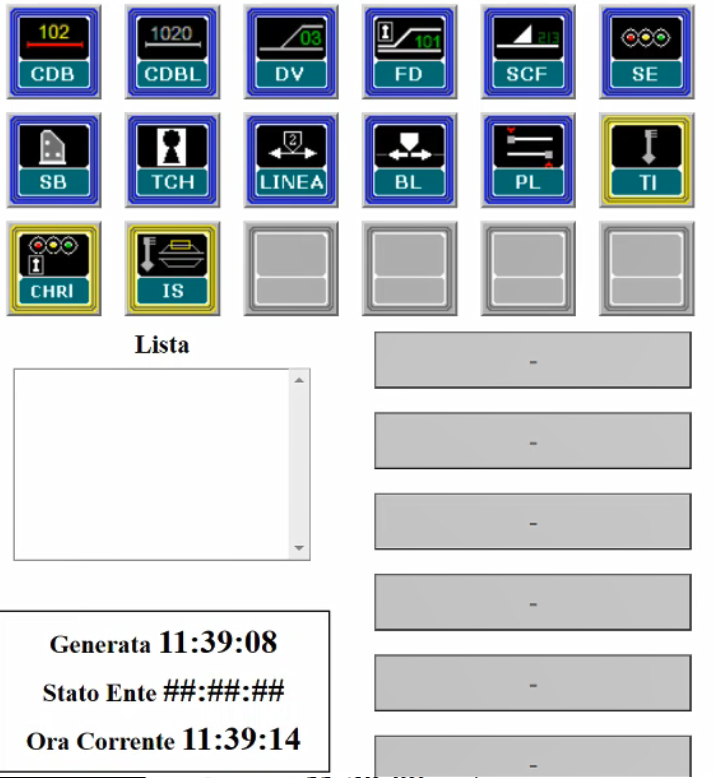
\includegraphics[scale=0.6]{img/interfaccia}
	\caption{Icone del Terminale Operatore}
\end{figure}
Quindi, le icone sono riportate in alto a sinistra e i relativi sottomen� vengono eventualmente generati dopo aver cliccato sul simbolo specifico.\\ La modalit� d'inoltro del comando pu� essere differenziata, infatti per alcuni comandi � richiesta la pressione dei tasti 0 - INVIO per confermare l'esecuzione, mentre altre volte, per i comandi critici, il comando deve essere autorizzato dal dirigente di movimento (DM) per diventare effettivo.
\newline
Nella sezione destra della schermata � possibile visualizzare una porzione del quadro luminoso relativa alla zona in cui l'agente di manutenzione sta effettuando le operazioni necessarie.\\
Nella schermata del Terminale Operatore viene riportata l'ora corrente insieme all'ora in cui � stato generato il quadro luminoso e lo stato dell'ente. Il quadro luminoso viene aggiornato periodicamente e l'ora dell'ultimo aggiornamento viene rappresentata in modo tale che l'operatore, confrontando l'ora corrente con l'ora in cui � stato generato il quadro luminoso, possa capire quanto le informazioni riportate siano attendibili.\\
Oltre al Terminale Operatore, tramite dei pulsanti riportati in alto a destra, � possibile accedere anche alla \textbf{schermata di Log} che offre informazioni sulle ultime operazioni eseguite, al \textbf{Piano schematico} e al \textbf{Quadro luminoso}, queste due schermate offrono ulteriori informazioni sullo stato del sistema.


\subsection{Il piano schematico}

Il \textbf{piano schematico} rappresenta senza il rispetto delle proporzioni la topografia di una stazione e riporta con un'apposita simbologia tutti gli enti di piazzale, sia relativi all'armamento che all'impianto di segnalamento, questi ultimi opportunamente numerati, nonch� altri elementi essenziali a caratterizzare la stazione per le esigenze della circolazione (fabbricato viaggiatori, marciapiedi, sottopassi pedonali, attraversamenti stradali, eventuali gallerie ecc.)\\
\begin{figure}[ht]
	\centering
	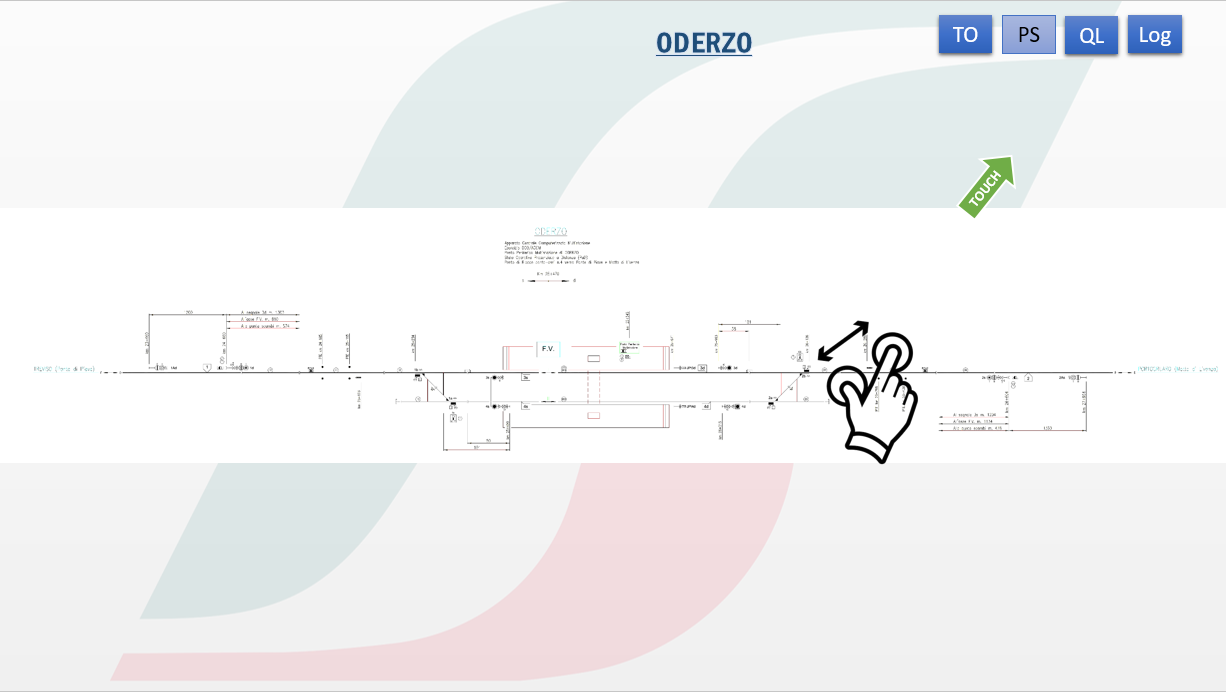
\includegraphics[scale=0.3]{img/pianoschematico}
	\caption{Piano schematico stazione di Oderzo}
\end{figure}

\subsection{Il quadro luminoso}

Il \textbf{quadro luminoso} prende il suo nome dalla possibilit� che gli � precipua di cambiare aspetto in alcune parti per indicare all'operatore la situazione degli itinerari dei treni, degli instradamenti delle manovre, della disposizione dei segnali, della posizione dei deviatori, dell'occupazione dei binari e quant'altro sia necessario per garantire regolarit� e sicurezza all'interno di una stazione ferroviaria. Questi controlli vengono offerti da lampadine poste dietro il quadro stesso che cambiano aspetto (acceso-spento) e attraverso filtri colorati rappresentano la situazione (SIL4) che si presenta nel piazzale della stazione. \cite{sette} \\
\begin{figure}[ht]
	\centering
	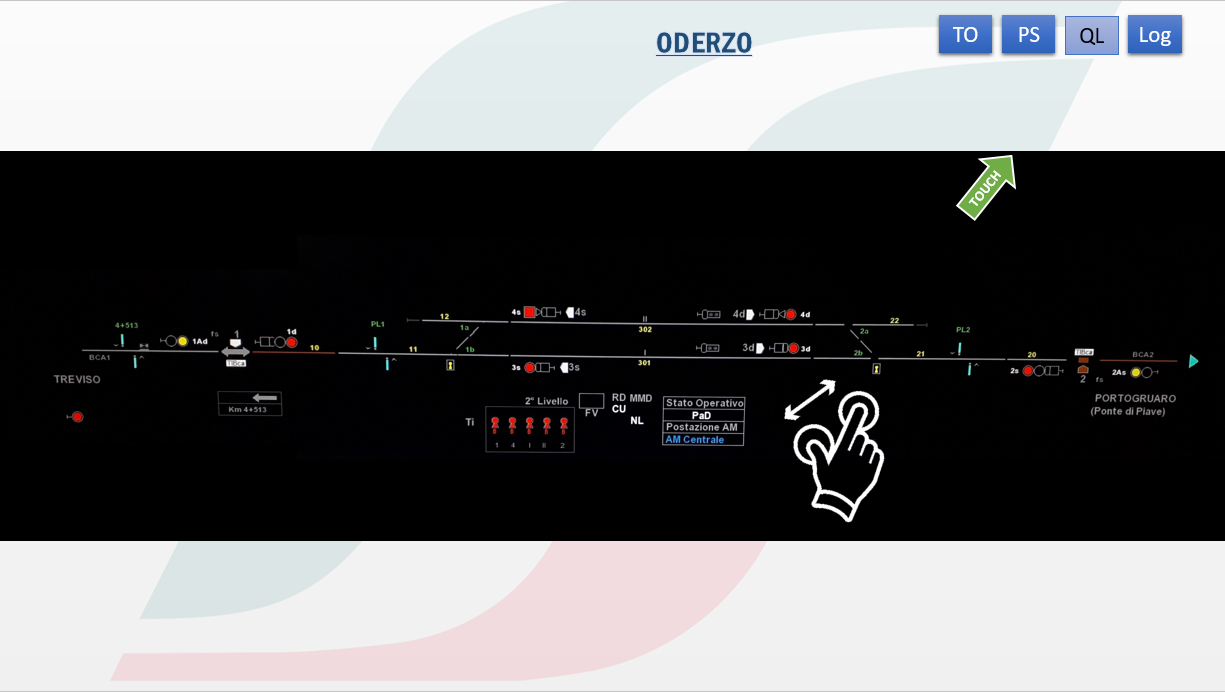
\includegraphics[scale=0.3]{img/quadrolumcom}
	\caption{Quadro luminoso stazione di Oderzo}
\end{figure}



\section{Schema funzionale}

Per riuscire a comprendere a pieno tutti i compiti e le operazioni che devono essere effettuate dai componenti presenti nell'apparato IMR � stato necessario utilizzare uno schema funzionale. Tale schema descrive graficamente tutti gli attori del sistema e i rispettivi ruoli: in verde sono riportati i componenti, in rosso i blocchi che descrivono le operazioni critiche e in blu i blocchi che descrivono le operazioni non critiche. 
\begin{figure}[htbp]
	\centering
	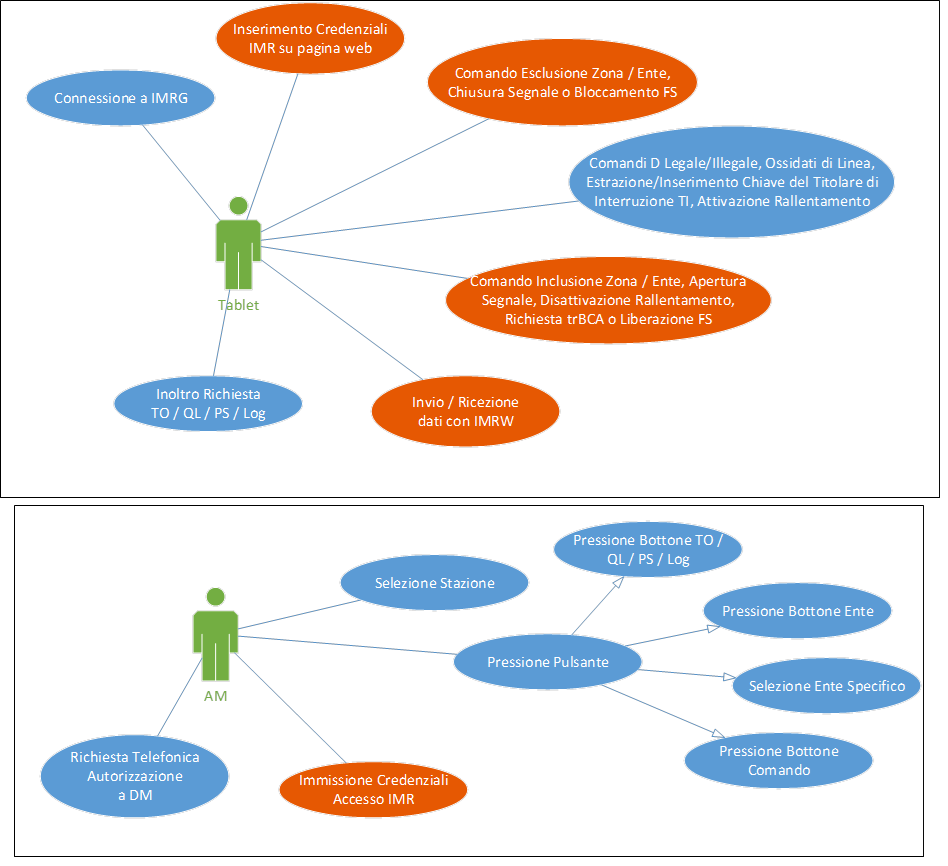
\includegraphics[scale=0.6]{img/schematablet}
	\caption{Schema funzionale Tablet Operatore e AM}
\end{figure}
\begin{figure}[htbp]
	\centering
	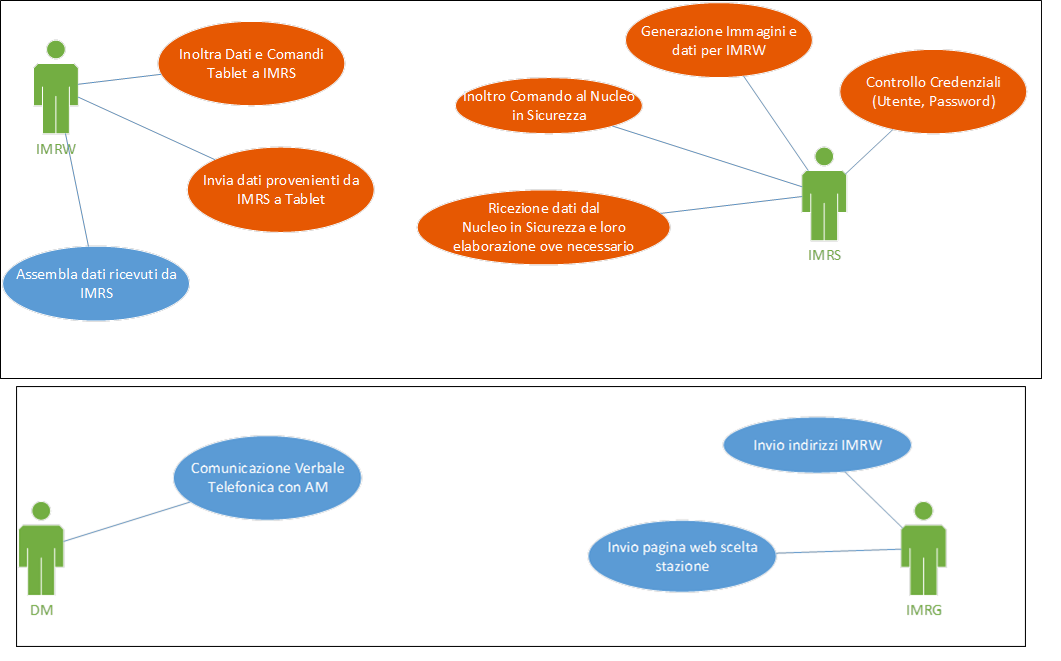
\includegraphics[scale=0.6]{img/schemaimrw}
	\caption{Schema funzionale IMRW, IMRS, DM e IMRG}
\end{figure}


\chapter{Hazard analysis dell'Apparato IMR}

In questo capitolo viene riportata l'analisi dei rischi vera e propria. Sono state studiate tutte le situazioni pericolose e i rischi associati e sono state individuate mitigazioni per permettere di ridurre la probabilit� di occorrenza degli hazards a un livello accettabile, aumentando la safety del sistema. Come suggerito dalla tecnica HAZOP, il sistema viene suddiviso in pi� parti e per ognuna di esse viene innanzitutto definito l'intento progettuale.\\
In seguito, vengono selezionati gli elementi delle parti e per ognuno di essi vengono applicate le parole guida elencate nei capitoli precedenti in ogni loro interpretazione. Se tale procedura evidenzia delle criticit�, verranno indagate le rispettive cause e conseguenze.\\
Per ogni rischio evidenziato verranno riportati la frequenza di occorrenza e la severit� dell'azzardo; dall'unione di queste due informazioni verr� ricavata la valutazione dell'azzardo in questione. Se il livello di rischio � trascurabile o tollerabile non sar� necessario individuare la mitigazione. Al contrario, se il livello del rischio � indesiderabile o intollerabile, verr� riportato un appropriato meccanismo di protezione o delle indicazioni atte a risolvere la problematica rilevata.\\Una volta che verranno applicate le interpretazioni di tutte le parole guida a tutti gli elementi progettuali, la sezione sar� contrassegnata come completata e si passer� ad esaminare le parti successive.\\ Tutte le informazioni relative all'Hazard analysis sono riportate in un file Excel con lo scopo di tener traccia di tutte le cause, conseguenze e mitigazioni rilevate. In tale file excel ogni azzardo viene contrassegnato in maniera univoca da un id in modo tale da riuscire a orientarsi nella tabella.\\

\section{Schema funzionale}

Per riuscire a comprendere a pieno tutti i compiti e le operazioni che devono essere effettuate dai componenti presenti nell'apparato IMR � stato necessario utilizzare uno schema funzionale. Tale schema descrive graficamente tutti gli attori del sistema e i rispettivi ruoli: in verde sono riportati i componenti, in rosso i blocchi che descrivono operazioni critiche e in blu i blocchi che descrivono operazioni non critiche. 
\begin{figure}[htbp]
	\centering
	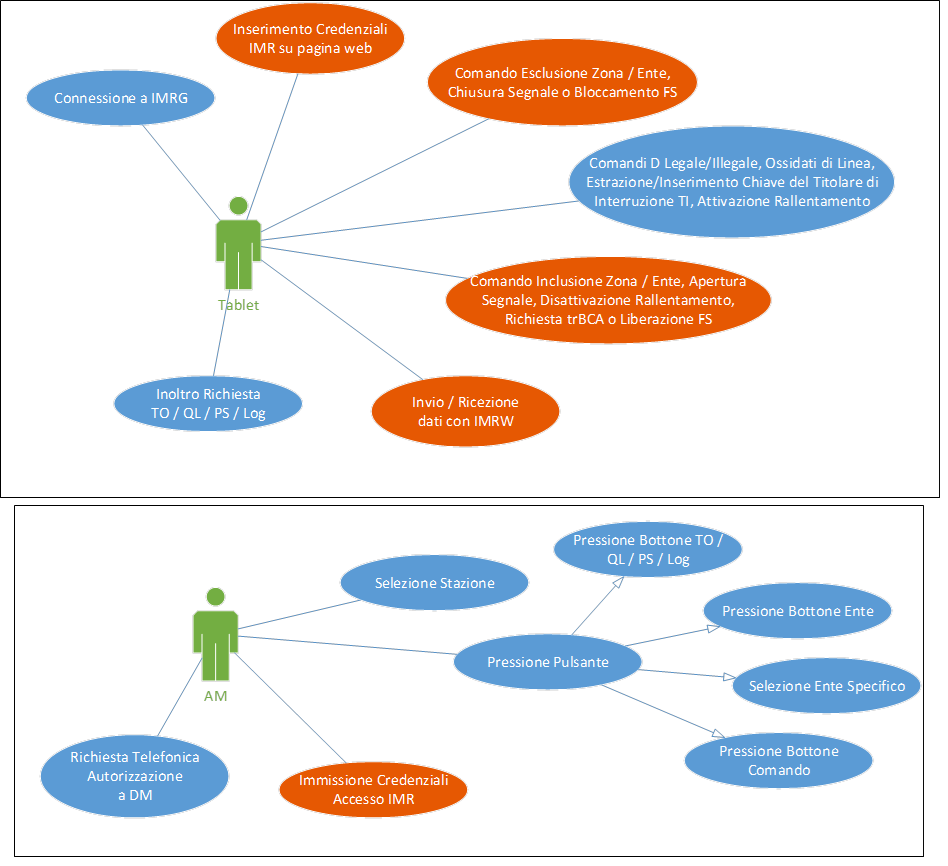
\includegraphics[scale=0.6]{img/schematablet}
	\caption{Schema funzionale Tablet Operatore e AM}
\end{figure}
\begin{figure}[htbp]
	\centering
	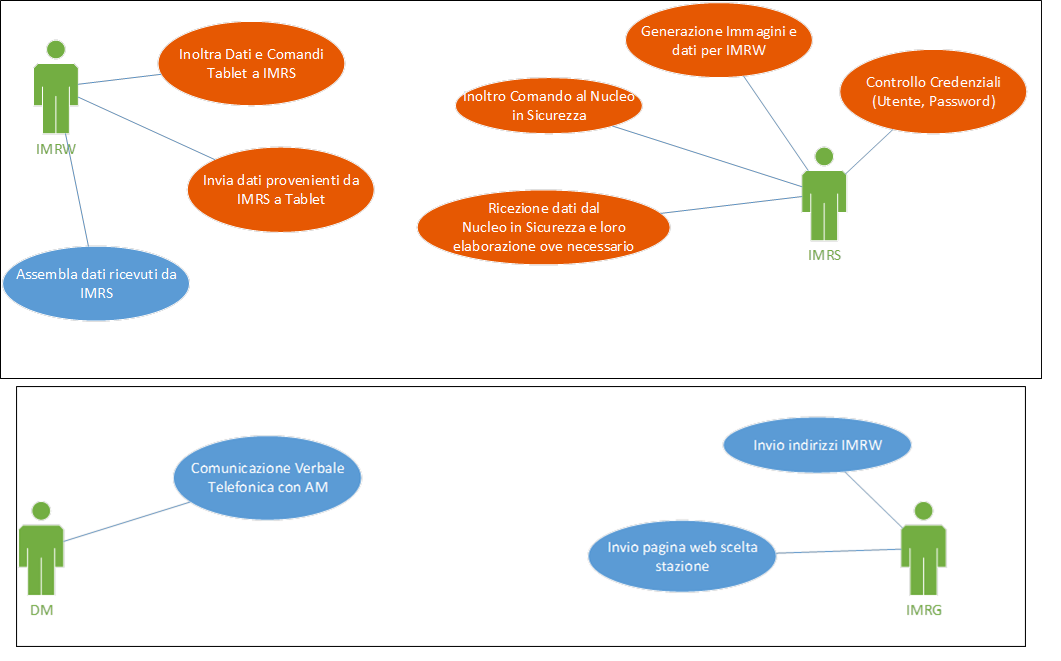
\includegraphics[scale=0.6]{img/schemaimrw}
	\caption{Schema funzionale IMRW, IMRS, DM e IMRG}
\end{figure}
\newline
\newline
\newline
\newline
\newline

\section{Autenticazione Tablet e Scelta Stazione}

La prima parte del sistema analizzata � quella relativa all'autenticazione sul Tablet e alla selezione della stazione d'interesse da parte dell'addetto manutenzione (AM).\\
Durante questa fase i componenti attivi sono: 
\begin{itemize}
	\item Addetto manutenzione;
	\item Tablet;
	\item Server IMRG;
	\item Server IRMW.
\end{itemize}
\begin{figure}
	\centering
	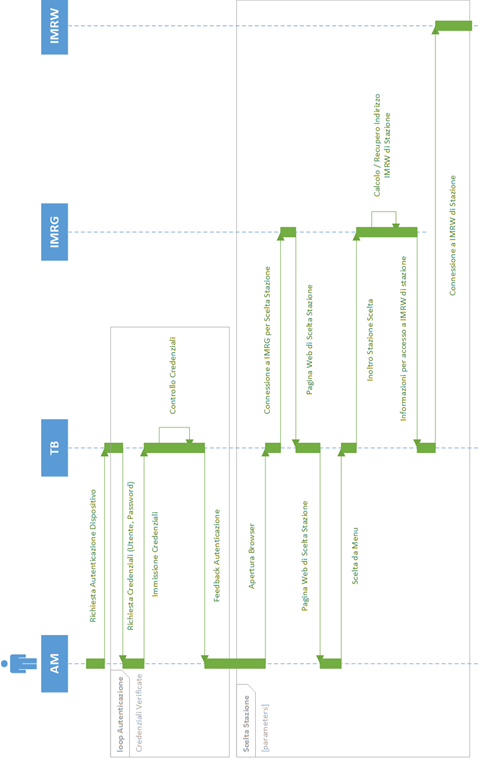
\includegraphics[scale=0.7]{img/sdprimo}
	\caption{Sequence Diagram prima fase}
\end{figure}
Come viene evidenziato dal sequence diagram questa sezione pu� essere divisa in due sottosezioni:
\begin{itemize}
	\item loop autenticazione;
	\item scelta stazione.
\end{itemize}
L'autenticazione al dispositivo � la prima operazione che l'addetto manutenzione deve effettuare, durante questa fase le credenziali vengono verificate direttamente dal Tablet.
Il server IRMG sar� presente solo in questa fase e nella successiva, in quanto il suo unico ruolo � quello di reindirizzare la connessione verso il server IRM locale e di memorizzare le chiavi pubbliche dell'AM. La reindirizzazione all'IMRW avviene immediatamente dopo la scelta della stazione da parte dell'addetto manutenzione.

\subsection{Rischi individuati}

Durante l'analisi di questa fase sono stati individuati vari rischi mediante l'utilizzo delle parole guida. Tale analisi ha evidenziato quasi tutti rischi \textit{tollerabili}, infatti molto spesso la severit� di suddetti rischi � stata classificata come \textit{insignificante}, in quanto gli azzardi non comportano problemi per la safety. Tra i rischi \textit{intollerabili} individuati in questa sezione del sequence diagram riportiamo il caso in cui l'AM venga reindirizzato su un server che potrebbe offrire un'interfaccia simile a quella attesa offerta da IMRG, ci� potrebbe indurre l'AM a condividere alcune informazioni personali come le credenziali per l'accesso. A questo punto il server dell'attaccante potrebbe funzionare da man-in-the middle tra l'AM ed il vero server.\\
\begin{figure}[htbp]
	\centering
	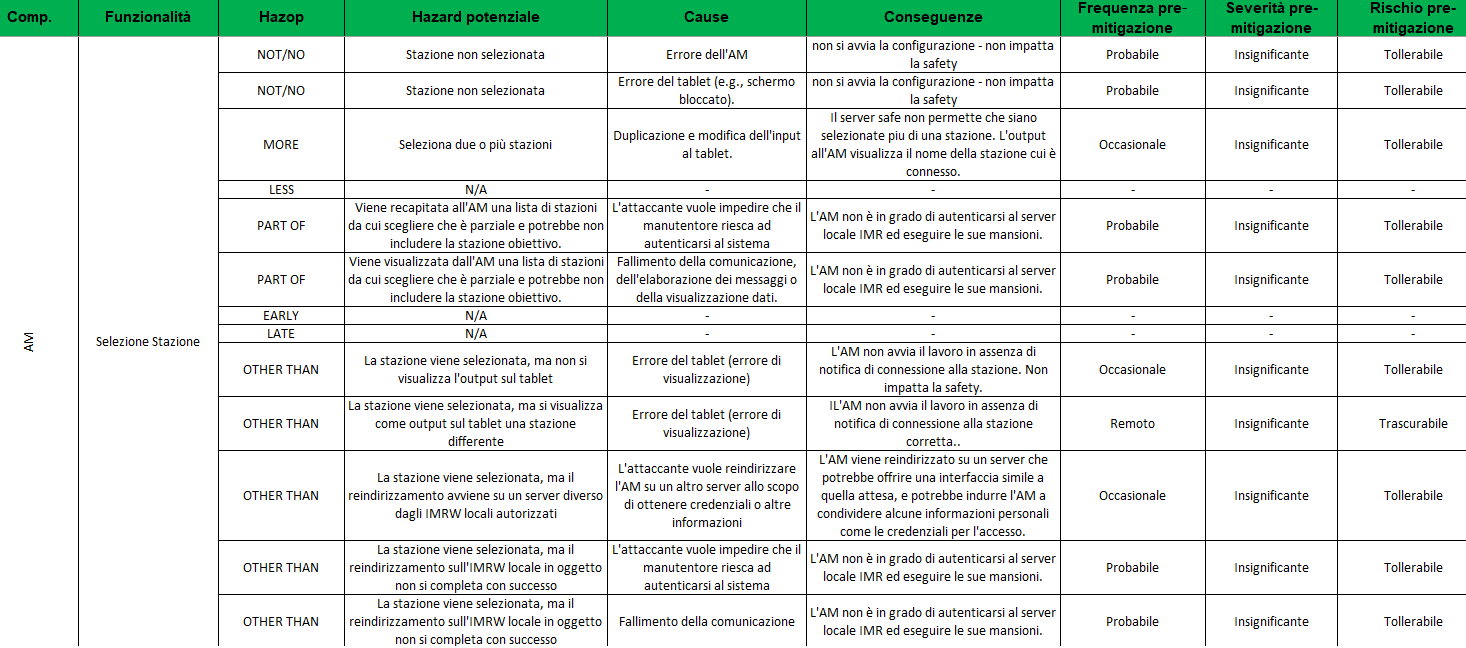
\includegraphics[scale=0.5]{img/exceluno}
	\caption{Sezione hazard analysis prima fase}
\end{figure}

\section{Login IMR}

\begin{figure}[htbp]
	\centering
	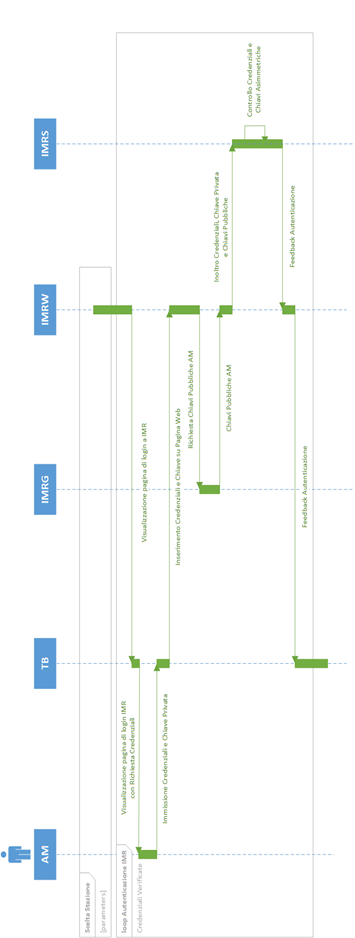
\includegraphics[scale=0.7]{img/sdsecondo}
	\caption{Sequence diagram seconda fase}
\end{figure}

Nella fase di autenticazione da parte dell'AM all'apparato IMR intervengono: 
\begin{itemize}
	\item Addetto manutenzione;
	\item Tablet;
	\item Server IMRG;
	\item Server IRMW;
	\item Server IMRS.
\end{itemize}
L'operazione di autenticazione coinvolge praticamente tutti i componenti dell'apparato IMR. Questa operazione avviene mediante ID/Password e un meccanismo di chiave asimmetrica (pubblica-privata). L'addetto manutenzione immette le proprie credenziali e la chiave privata, la chiave pubblica � invece memorizzata dal server centrale IMRG che ha il compito di inviarla all'IMRW. Il server IMRW inoltra tutte le informazioni relative all'autenticazione al server IMRS che si occuper� di verificare l'effettiva correttezza di quest'ultime e quindi di inviare la schermata del Terminale Operatore al Tablet se l'utente � autorizzato. IMRS � un server sicuro, progettato, sviluppato e certificato SIL4 ed � per questo che il controllo delle credenziali viene effettuato su quest'ultimo e non su IMRW.

\subsection{Rischi seconda parte}
I rischi individuati in questa sezione non coinvolgono la safety del sistema. Se l'AM non riesce ad autenticarsi all'IMR locale e quindi non riesce a svolgere le sue mansioni per qualunque causa (errore umano, errore accidentale sul server, attacco esterno ecc..), si verifica un problema per la availability e la security del sistema ma non per la safety, quindi tali rischi vengono classificato come \textit{tollerabili}.

\begin{figure}[htbp]
	\centering
	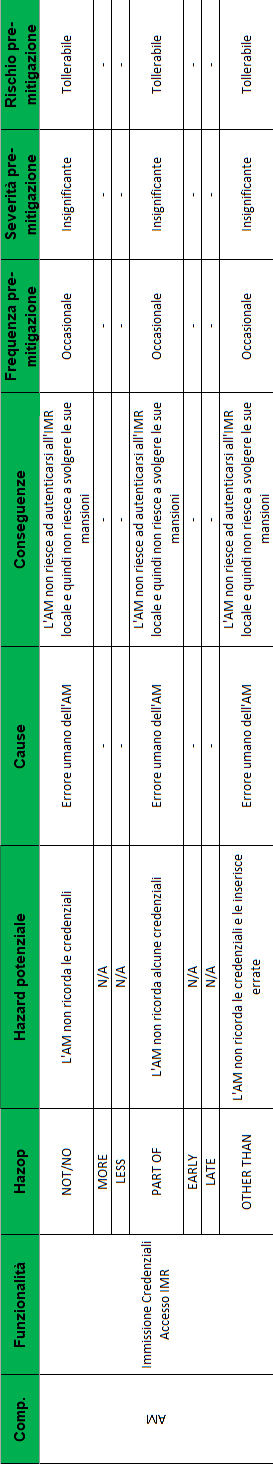
\includegraphics[scale=0.5]{img/exceldue}
	\caption{Sezione hazard analysis seconda fase}
\end{figure}

\section{Visualizzazione Terminale Operatore (TO)}

\begin{figure}[htbp]
	\centering
	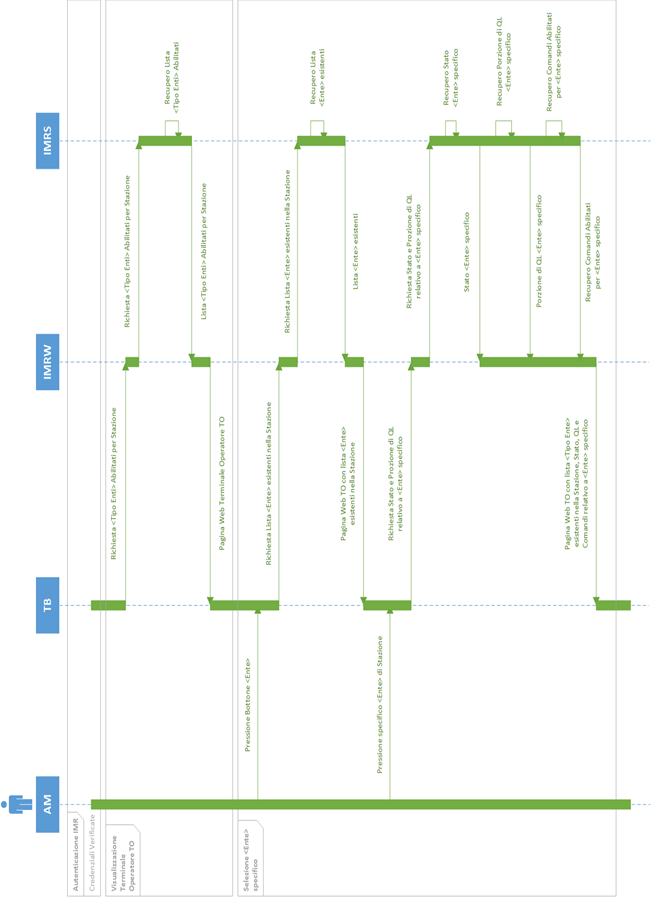
\includegraphics[scale=0.7]{img/sdterzo}
	\caption{Sequence diagram terza fase}
\end{figure}

Durante le operazioni relative a questa fase intervengono i seguenti componenti: 
\begin{itemize}
	\item Addetto manutenzione;
	\item Tablet;
	\item Server IRMW;
	\item Server IMRS.
\end{itemize}

Anche qui, � possibile rilevare due sottosezioni:
\begin{itemize}
	\item visualizzazione Terminale Operatore TO;
	\item selezione <Ente> specifico.
\end{itemize}
Infatti, dopo aver verificato la correttezza delle credenziali, viene inviata dall'IMRS al Tablet la pagina web del Terminale Operatore che riporta tutti gli Enti abilitati per quella determinata stazione.\\ L'addetto manutenzione pu� quindi iniziare a inviare i comandi opportuni per le operazioni di manutenzione. L'AM in questa fase � in grado di premere i bottoni degli <Enti> di stazione e l'IMRS inoltrer� la relativa pagina Web TO con lista <Tipo Ente> esistenti nella Stazione, Stato, QL, e i comandi relativi all'Ente specifico.


\subsection{Rischi terza parte}


\section{Esecuzione comando AM}

NON VA BENE IL SEQUENCE DIAGRAM

\section{Selezione Piano Schematico (PS), Quadro Luminoso (QL), Log}

\chapter{Mitigazioni}

Nel capitolo precedente sono stati analizzati i principali azzardi individuati nell'apparato IMR. La valutazione ha classificato molti azzardi come \textit{intollerabili}, per questi ultimi � opportuno individuare una procedura di mitigazione. La mitigazione pu� avere come scopo quello di ridurre la severit� dell'azzardo oppure la frequenza, in modo tale che possa venir considerato \textit{tollerabile} per il sistema. Di seguito sono riportate le mitigazioni applicate all'apparato in seguito all'hazard analysis.


\section{Utilizzo di una One Time Password}
Dall'analisi � risultato che la maggior parte della situazioni indesiderabili si verificherebbe quando l'AM tenta di eseguire un comando critico. Infatti � possibile che a causa di un attacco esterno oppure accidentalmente, il messaggio contenente il comando venga eliminato o alterato, cos� come la risposta di conferma esecuzione del comando.Per ovviare a tale problematica � stato pensato di aggiungere all'architettura dell'apparato un ulteriore dispositivo: lo Smartphone.\\
Tale dispositivo viene impiegato dal sistema quando l'AM ha intenzione di eseguire un comando critico per la sicurezza, con lo scopo di utilizzare un canale alternativo per convalidare il comando.\\ In particolare, quando l'AM decide di effettuare un comando critico, l'IMRS invia la richiesta di conferma del comando al Tablet; per attuare tale operazione, l'AM deve inserire sul Tablet una One Time Password pervenuta intanto sullo Smartphone tramite un canale alternativo. Quindi una volta che l'IMRS riceve la richiesta di esecuzione di un comando critico, risponde con:
\begin{itemize}
	\item al Tablet: una immagine contenente il comando ricevuto, incluse alcune informazioni associate;
	\item allo Smartphone: una informazione contenente il comando ricevuto e una OTP.
\end{itemize}
\begin{figure}[ht]
	\centering
	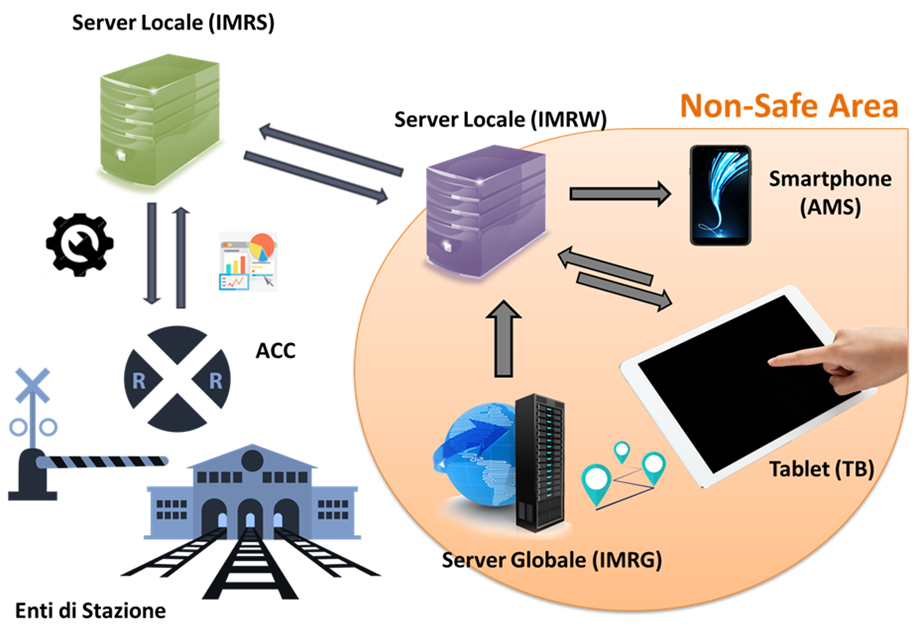
\includegraphics[width=0.7\linewidth]{img/architdue}
	\caption{Il ruolo dello Smartphone nell'apparato IMR}
\end{figure}
In questo modo l'AM pu� verificare la consistenza delle informazioni giunte su Tablet e Smartphone e in seguito inserire la OTP sul Tablet per confermare il comando. A questo punto il server IMRS potr� inoltrare il comando al nucleo in sicurezza, se la password risulta verificata.\\ Se il nucleo esegue il comando, viene costruita e inviata da IMRS:
\begin{itemize}
	\item al Tablet: una immagine che contiene la conferma del comando (o le informazioni richieste) e una nuova OTP;
	\item allo Smartphone: la stessa OTP e le informazioni accessorie per confermare i dati contenuti nell'immagine.
\end{itemize}
Attraverso questa procedura � possibile contrastare eventuali contraffazioni alle informazioni eseguite da un attaccante.\\
Invece, se il nucleo non esegue il comando, viene inviata una notifica solo verso il Tablet, senza OTP. Non avendo OTP da inserire, l'AM ne conclude che il comando non � stato eseguito.\\
Durante tutta la procedura appena descritta l'AM � direttamente responsabile di confrontare visivamente che le informazioni giunte sui dispositivi combacino, incluse le OTP. L'AM inoltre � anche responsabile di non assumere la corretta esecuzione del comando, qualora la procedura realizzata devii dallo schema descritto.\\ Nell'immagine seguente � possibile osservare il sequence diagram della fase \textit{Esecuzione comando} con gli aggiornamenti riguardanti l'aggiunta dell'utilizzo della OTP.
\begin{figure}[ht]
	\centering
	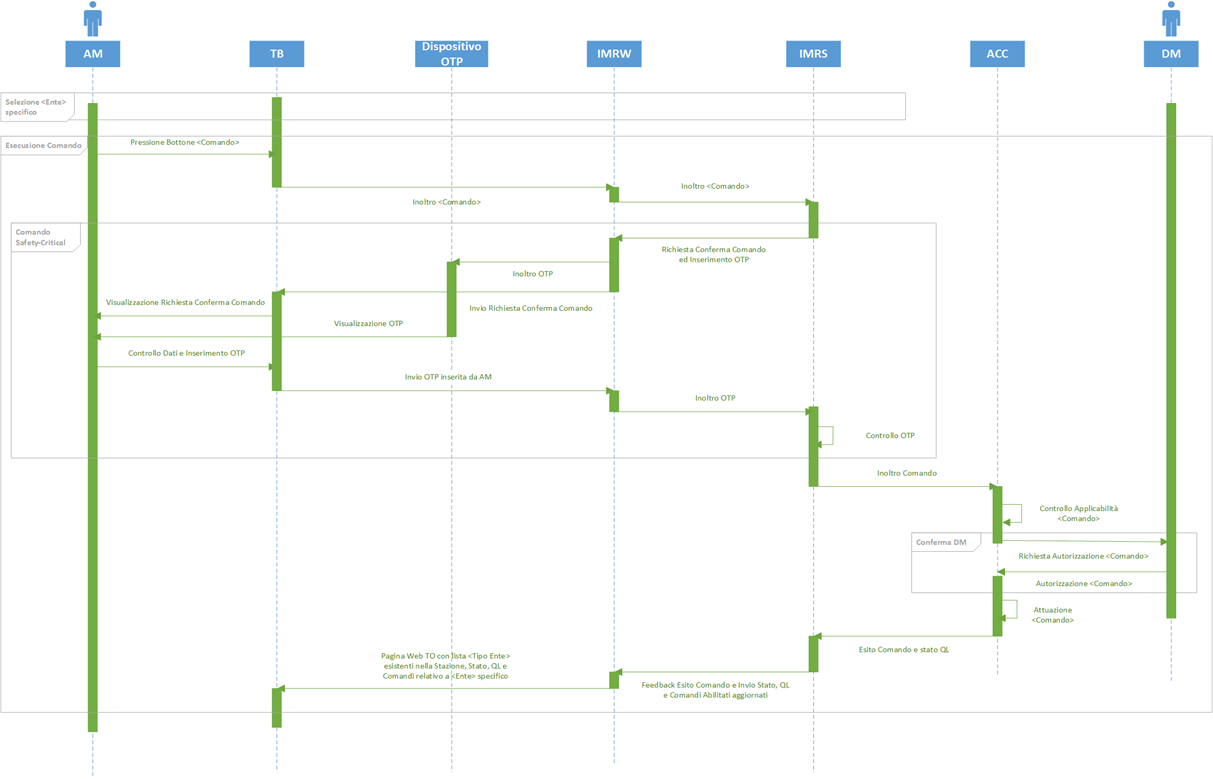
\includegraphics[width=0.9\linewidth]{img/sdesecuzione}
	\caption{Sequence diagram Esecuzione comando}
\end{figure}


\section{Utilizzo del protocollo PVS}
Poich� i canali di comunicazione ordinari non sono affidabili, l'apparato IMR adotta un protocollo noto come Protocollo Vitale Standard (PVS), ideato da RFI per consentire interazioni sicure tra diversi dispositivi. Per imporre la safety di tutte le comunicazioni la procedura deve essere progettata secondo lo standard EN50159 \cite{dodici} e dovrebbe essere codificata come linguaggio di medio-basso livello in accordo allo standard EN50128 \cite{tredici}.\\ Il protocollo PVS fornisce un livello di safety insieme alla protezione contro l'accesso non autorizzato attraverso l'uso di codici di sicurezza e tecniche crittografiche. Le tecniche e gli algoritmi inclusi nel protocollo sono stati identificati tra quelli collaudati, validati e proven-in-use nel settore ferroviario.
\newline
Il protocollo pu� essere riassunto come un software aggiuntivo che fornisce le funzionalit� OSI di sessione e presentazione tramite:
\begin{itemize}
	\item codici di sicurezza (per garantire l'integrit� del messaggio);
	\item numero di sequenza (per evitare la re-sequenziazione, ripetizione, inserimento e cancellazione di messaggi);
	\item execution cycle (per ottenere la freshness del messaggio);
	\item identificativi di nodo, sorgente e destinazione, univoci (per l'autenticit�);
	\item crittografia.
\end{itemize}
Dall'unione di questi meccanismi � possibile garantire comunicazioni sicure.
\newline
La comunicazione bidirezionale tra IMRS e IMRW � condotta tramite messaggi scambiati attraverso il protocollo PVS, quindi entrambi i server dovranno aprire un canale di comunicazione bidirezionale.\\
Invece l'interazione tra il server IMRW e il Tablet prevede una procedura pi� articolata:
\begin{itemize}
	
 \item il server genera delle pagine HTML tramite opportuno linguaggio di scripting lato-server;
 \item questo flusso HTTP viene intercettato da uno script, il PVS Server, che prende il messaggio e lo usa come payload per una comunicazione PVS. Il messaggio PVS cos� creato viene inviato al Tablet su una porta predefinita sulla quale ascolta il modulo PVS Client. 
 \item il modulo PVS Client, dopo aver ricevuto i dati PVS, li decapsula e li reinoltra sulla porta HTTP (default: 80) del Tablet. 
\end{itemize}
 Quando l'AM vuole inviare dei comandi tramite TB al server IMRW, verr� eseguito il procedimento a ritroso, sfruttando lo stesso canale sicuro.
 \begin{figure}[ht]
 	\centering
 	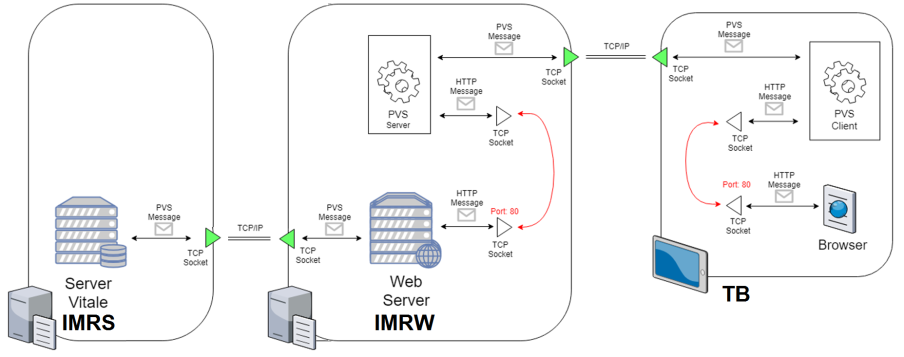
\includegraphics[width=0.9\linewidth]{img/pvs}
 	\caption{Protocollo PVS}
 \end{figure}
 

\section{Alcune buone pratiche}
Tramite l'utilizzo delle due mitigazioni appena descritte, tutti i rischi classificati come \textit{intollerabili} nel capitolo precedente, possono venir rivalutati e considerati invece come \textit{ammissibili} per l'apparato IMR. Infatti, attraverso l'uso del protocollo PVS e della procedura che prevede l'inserimento delle OTP, la safety del sistema non � pi� a rischio. \\
Di seguito ho pensato di inserire alcune buone pratiche per l'utilizzo del sistema, per cercare di ottimizzare l'impiego di quest'ultimo:
\begin{itemize}
	\item \textit{avere a disposizione un tablet di riserva}: questo accorgimento � necessario quando il tablet utilzzato dall'operatore non riesce a eseguire correttamente le operazioni di base (touchscreen non reattivo, spegnimento improvviso del tablet, mancata gestione della batteria ecc..);
	
	\item \textit{riaggiornamento pagina}: da effettuare quando ad esempio la lista delle stazioni non � completa;
	
	\item \textit{utilizzare password potenti}: per fare in modo che il meccanismo di autenticazione tramite password sia solido e sia difficile per un attaccante introdursi nel sistema � necessario che la password adottata sia pi� complessa possibile. E' quindi consigliabile utilizzare sia lettere maiuscole che minuscole, segni e numeri;
	
	\item \textit{numero tentativi autenticazione limitati}: � possibile che un attaccante per accedere al sistema abbia intenzione di provare tutte le password di un dizionario. Per evitare che tale attacco sia possibile, � necessario imporre che i tentativi di autenticazione siano limitati, ad esempio un numero appropriato di tentativi di autenticazione potrebbe essere pari a 3;
	
	\item \textit{modificare la password periodicamente}: per garantire la sicurezza del sistema � opportuno che le passoword degli addetti manutenzione vengano modificate periodicamente;
	
	\item \textit{memorizzare la chiave privata in sicurezza}: per evitare che il file contente la chiave privata possa essere reperibile da individui non autorizzati ad accedere al sistema � opportuno che venga salvato in una posizione di massima sicurezza;

	\item \textit{effettuare l'autenticazione periodicamente}: per fare in modo che il Tablet non possa essere utilizzato da terzi per l'esecuzione di comandi, sarebbe bene che periodicamente debba essere effettuata l'operazione di login da parte dell'AM.


\end{itemize}

\begin{thebibliography}{99}

\bibitem{uno}{Wikipedia - \emph{FMEA}}

\bibitem{due}{Andrea Bondavalli - \emph{Analisi quantitativa dei Sistemi Critici}}

\bibitem{tre}{Wikipedia - \emph{HAZOP}}

\bibitem{quattro}{www.analisideirischinformatici.it - \emph{ANALISI DEI RISCHI INFORMATICI E POLICY SULLA SICUREZZA AZIENDALE}}

\bibitem{cinque}{http://www.rfi.it - \emph{Apparati Centrali}}

\bibitem{sei}{http://www-3.unipv.it- \emph{Circolazione ed Impianti di Sicurezza e Segnalamento}}

\bibitem{sette}{Wikipedia - \emph{Quadro luminoso}}

\bibitem{otto}{IlSole24Ore - \emph{Storia quasi breve del risk management nelle banche}}


\bibitem{nove}{Andrea Ceccarelli, Mohamad Gharib, Andrea Bondavalli, Tommaso Zoppi - \emph{Specifica Architettura IMR}}


\bibitem{dieci}{Wikipedia - \emph{Dependability}}

\bibitem{undici}{Lorenzo Falai - \emph{Certification of Critical Systems}}

\bibitem{dodici}{CENELEC - \emph{EN. "50159." Railway applications-Communication, signalling and processing systems-Safety-related communication in transmission Part 2 (2001)}}

\bibitem{tredici}{CENELEC - \emph{EN 50128, "Railway applications - Communication, signalling and processing systems - Software for railway control and protection systems}}

\end{thebibliography}

%--------------------------------------------------------------
\end{document}
%--------------------------------------------------------------
